\subsection{Point distributions}

In this section, X denotes a manifold of class \(C^{r}\) , and x is a point of X.

13.2.1. Let \(\mathcal{A}\) be the set of pairs \((c, t)\) , where \(c = (\mathrm{U}, \varphi, \mathrm{E})\) is a chart of X centered at \(x\) , and where \(t \in \mathrm{TS}^{(r)}(\mathrm{E})\) . Two elements \(((\mathrm{U}, \varphi, \mathrm{E}), t)\) and \(((\mathrm{U}', \varphi', \mathrm{E}'), t')\) of \(\mathcal{A}\) are said to be equivalent if \(t' = \gamma_*(t)\) , where \(\gamma = \varphi' \circ \varphi^{-1}\) . One thus obtains an equivalence relation on \(\mathcal{A}\) ; an equivalence class for this relation is called a point distribution at \(x\) on X.

Let \(\mathrm{T}_{x}^{(r)}(\mathrm{X})\) be the set of point distributions at x on X. If c is a chart of X centered at x, the map

\[
\theta_ {c} \colon \mathsf {T S} ^ {(r)} (\mathrm{E}) \to \mathbf {T} _ {x} ^ {(r)} (\mathrm{X})
\]

which maps \(t\) to the class of \((c, t)\) , is a bijection. In all that follows, we equip \(\mathrm{T}_{x}^{(r)}(\mathrm{X})\) with the structure of a K-vector space obtained by transporting that of \(\mathrm{TS}^{(r)}(\mathrm{E})\) by \(\theta_{c}\) ; this structure does not depend on the choice of \(c\) . Similarly, if \(k \leqslant r\) , we denote by \(\mathrm{T}_{x}^{(k)}(\mathrm{X})\) and \(\mathrm{T}_{x}^{(k)+}(\mathrm{X})\) the images of \(\mathrm{TS}^{(k)}(\mathrm{E})\) and \(\mathrm{TS}^{(k)+}(\mathrm{E})\) under \(\theta_{c}\) ; they do not depend on the choice of \(c\) . An element of \(\mathrm{T}_{x}^{(r)}(\mathrm{X})\) is said to be of order \(\leqslant k\) if it belongs to \(\mathrm{T}_{x}^{(k)}(\mathrm{X})\) . One has

\[
\mathbf {T} _ {x} ^ {(k)} (\mathbf {X}) = \mathbf {T} _ {x} ^ {(0)} (\mathbf {X}) \oplus \mathbf {T} _ {x} ^ {(k) +} (\mathbf {X}).
\]

There exists one and only one element \(\varepsilon_x\) of \(\mathrm{T}_x^{(0)}(\mathbf{X})\) such that we have \(\theta_c(1) = \varepsilon_x\) for every chart \(c\) of \(\mathbf{X}\) centered at \(x\) . If \(t\) is a point distribution in \(x\) , we call the constant term of \(t\) the element \(\lambda\) of \(\mathbf{K}\) such that \(t - \lambda \varepsilon_x \in \mathrm{T}_x^{(r)+}(\mathbf{X})\) ; we say that \(t\) is without constant term if its constant term is zero.

13.2.2. Let F be a separated polynomial space, and let f be a function of class \(C^{r}\) with values in F, defined on a neighborhood of x. Let t be a point distribution at x on X.

Consider a map \(c = (\mathrm{U}, \varphi, \mathrm{E})\) of X centered at \(x\) , and set \(f_c = f \circ \varphi^{-1}\) and \(t_c = \theta_c^{-1}(t)\) ; the element \(\langle f_c, t_c \rangle\) of F defined in 13.1.3 does not depend on the choice of \(c\) ; we denote it \(\langle f, t \rangle\) . One has \(\varepsilon_x(f) = f(x)\) . \(^{(1)}\) The constant term of \(t\) is \(\langle 1, t \rangle\) .

If \(\mathbf{F}'\) is a separated polynormed space and if \(u: \mathbf{F} \to \mathbf{F}'\) is continuous and linear, we have \(\langle u \circ f, t \rangle = u(\langle f, t \rangle)\) .

Suppose that F is a Banach space, and that t is of order \(\leqslant k\) , with k finite. Let \(j \in \mathrm{J}_{x}^{k}(\mathrm{X}, \mathrm{F})\) , cf. 12.1.2, and let \(f \in j\) . Then \(\langle f, t \rangle\) depends only on the jet j; it is denoted \(\langle j, t \rangle\) . The map from \(\mathrm{T}_{x}^{(k)}(\mathrm{X}) \times \mathrm{J}_{x}^{k}(\mathrm{X}, \mathrm{F})\) to F thus defined is bilinear. When F = K, we have set \(\mathrm{J}_{x}^{k}(\mathrm{X}, \mathrm{F}) = \mathrm{P}_{x}^{k}(\mathrm{X})\) , cf. 12.6.2, and we obtain a bilinear form on \(\mathrm{T}_{x}^{(k)}(\mathrm{X}) \times \mathrm{P}_{x}^{k}(\mathrm{X})\) .

13.2.3. Let \(\varphi: X \to Y\) be a morphism of manifolds of class \(C^r\) and let \(y = \varphi(x)\) . Let \(c = (U, \psi, E)\) be a chart of \(X\) centered at \(x\) and let \(c' = (U', \psi', E')\) be a chart of \(Y\) centered at \(y\) ; let \(\bar{\varphi}\) be the expression of \(\varphi\) in these charts (5.3.2), and let \(\bar{\varphi}_*\) be the corresponding map from \(\mathrm{TS}^{(r)}(E)\) to \(\mathrm{TS}^{(r)}(E')\) , cf. 13.1.4. There exists one and only one linear map, denoted \(\mathrm{T}_x^{(r)}(\varphi)\) or \(\varphi_*\) , from \(\mathrm{T}_x^{(r)}(X)\) to \(\mathrm{T}_y^{(r)}(Y)\) making the diagram commutative

\pandocbounded{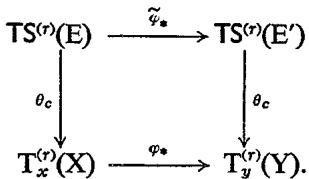
\includegraphics[keepaspectratio]{images/part001_e22e7577.jpg}}

This map does not depend on the choice of \(c\) and \(c'\) . If \(t \in \mathrm{T}_{x}^{(r)}(\mathbf{X})\) , one says that \(\varphi_{*}(t)\) is the image of \(t\) by \(\varphi\) . One has \(\varphi_{*}(\varepsilon_{x}) = \varepsilon_{y}\) . If \(k \leqslant r\) , one has

\[
\varphi_ {*} (\mathrm{T} _ {x} ^ {(k)} (\mathrm{X})) \subset \mathrm{T} _ {y} ^ {(k)} (\mathrm{Y}) \quad \text { and } \quad \varphi_ {*} (\mathrm{T} _ {x} ^ {(k) +} (\mathrm{X})) \subset \mathrm{T} _ {y} ^ {(k) +} (\mathrm{Y}).
\]

If \(\varphi': X \to Y\) is a morphism of class \(C^r\) such that \(\varphi'(x)=y\) , one has \(\varphi_* = \varphi_*'\) if and only if \(j_x^r(\varphi) = j_x^r(\varphi')\) , cf. 12.1.

If \(\varphi\) is an immersion (resp. a submersion) at \(x, \varphi_*\) is injective (resp. surjective); the converse is true if \(\dim_y Y < +\infty\) .

If \(\varphi'\colon\mathbf{Y}\to\mathbf{Z}\) is a morphism of manifolds of class \(\mathbf{C}^{r}\) and if \(t\in\mathbf{T}_{x}^{(r)}(\mathbf{X})\) , one has \((\varphi'\circ\varphi)_{*}(t)=\varphi_{*}^{\prime}(\varphi_{*}(t))\) .

Let F be a separated polynormed space, and let f be a function of class \(C^{r}\) with values in F, defined in a neighborhood of y. We then have

\[
\langle f, \varphi_ {*} (t) \rangle = \langle f \circ \varphi , t \rangle \quad \text {   for   all   } \quad t \in \mathrm{T} _ {x} ^ {(r)} (\mathrm{X}).\tag{1}
\]

For \(t\) given, the relations (1) (for \(f\) and \(F\) variables) characterize \(\varphi_{*}(t)\) ; when \(\dim_y Y < +\infty\) , one may restrict oneself to \(F = K\) .

13.2.4. Suppose that X is an open submanifold of a Banach space E. Denote by \(\varphi_x\) the map \(y \mapsto y - x\) from X into E; the chart \(c = (X, \varphi_x, E)\) is centered at \(x\). We then identify \(\mathrm{T}_x^{(r)}(\mathbf{X})\) with \(\mathrm{TS}^{(r)}(\mathbf{E})\) by means of \(\theta_c^{-1}\). In particular, we have \(\mathrm{T}_x^{(\infty)}(\mathbf{X}) = \mathrm{TS}(\mathbf{E})\) .

Let F be a Banach space, let \(u: E \to F\) a continuous linear map, and let \(x \in E\) , \(y \in F\) such that \(u(x) = y\) . Identify as above \(\mathrm{T}_{x}^{(\infty)}(E)\) with TS(E) and \(\mathrm{T}_{y}^{(\infty)}(F)\) with TS(F). The map

\[
u _ {*} \colon \mathrm{TS(E)} \rightarrow \mathrm{TS(F)} \quad (\text { cf. } 13.2.3)
\]

coincides with the map TS(u) induced by the canonical extension of u to the tensor algebra.

13.2.5. If \(k \leqslant r\) , one denotes by \(\mathrm{T}^{(k)}(\mathrm{X})\) (resp. \(\mathrm{T}^{(k)+}(\mathrm{X})\) ) the set sum of \(\mathrm{T}_a^{(k)}(\mathrm{X})\) (resp. of \(\mathrm{T}_a^{(k)+}(\mathrm{X})\) ) for \(a \in \mathrm{X}\) . A map \(t: \mathrm{X} \to \mathrm{T}^{(k)}(\mathrm{X})\) such that \(t(a) \in \mathrm{T}_a^{(k)}(\mathrm{X})\) for all \(a \in \mathrm{X}\) is called a field of point distributions of order \(\leqslant k\) .

Suppose \(k\) is finite and X is locally of finite dimension. For every \(a \in X\) , the bilinear form \((j, t) \mapsto \langle j, t \rangle\) (cf. 13.2.2) defines an isomorphism \(i_a\) of \(\mathrm{T}_a^{(k)}(\mathrm{X})\) onto the dual \(\mathrm{P}_a^k(\mathrm{X})^*\) of \(\mathrm{P}_a^k(\mathrm{X})\) . The \(i_a\) define a bijection \(i: \mathrm{T}^{(k)}(\mathrm{X}) \to \mathrm{P}^k(\mathrm{X})^*\) , where \(\mathrm{P}^k(\mathrm{X})^*\) denotes the dual of the vector bundle \(\mathrm{P}^k(\mathrm{X})\) ; by transport of structure via \(i^{-1}\) , one endows \(\mathrm{T}^{(k)}(\mathrm{X})\) with a vector bundle structure with base X and class \(\mathbf{C}^{r-k}\) . A field of point distributions of order \(\leqslant k\) is said to be of class \(\mathbf{C}^s\) , with \(s \leqslant r - k\) , if it is a section of class \(\mathbf{C}^s\) of the bundle \(\mathrm{T}^{(k)}(\mathrm{X})\) .

Let \(\varphi\colon\mathbf{X}\to\mathbf{Y}\) be a morphism of manifolds of class \(\mathbf{C}^{r}\) and suppose that Y, like X, is locally finite-dimensional. Then \(\varphi_{*}\colon\mathrm{T}^{(k)}(\mathrm{X})\to\mathrm{T}^{(k)}(\mathrm{Y})\) is a \(\varphi\) -morphism of vector bundles of class \(\mathbf{C}^{r-k}\) .

13.2.6. Let \(k\) be an integer such that \(0 \leqslant k \leqslant r\) . If U is an open set of a finite-dimensional Banach space E, the vector bundle \(\mathbf{T}^{(k)}(\mathbf{U})\) is identified, by virtue of 13.2.4, with the trivial bundle with fibre \(\mathbf{TS}^{(k)}(\mathbf{E})\) .

Take in particular \(E = K^n\) , with \(n \geqslant 0\) , and let \((e_1, \ldots, e_n)\) be the canonical basis of \(E\) . If \(\alpha = (\alpha_1, \ldots, \alpha_n)\) is an element of \(N^n\) , denote by \(\Delta^\alpha\) the element \(\gamma_{\alpha_1}(e_1) \ldots \gamma_{\alpha_n}(e_n)\) of \(TS(E)\) (the product used being the symmetric product of symmetric tensors, cf. A, IV, § 5, no. 3). \(^{(1)}\) The \(\Delta^\alpha\) , for \(|\alpha| \leqslant k\) , form a basis of \(TS^{(k)}(E)\) ; if \(a \in K^n\) , one denotes by \(\Delta_a^\alpha\) the corresponding elements of \(T_a^{(k)}(E)\) . Let F be a separated polynormed space, and f a function of class \(C^r\) , with values in F, defined in a neighbourhood of \(a\) ; if \(\alpha \in N^n\) , the element \(\langle f, \Delta_a^\alpha \rangle\) coincides with the element \((\Delta^\alpha f)(a)\) defined in 2.5.3, 3.2.1 and 4.2.1.

Suppose X is locally finite-dimensional, and let \(\xi = (\xi^1, \ldots, \xi^n)\) be a coordinate system of X in an open set U. If \(a \in \mathbf{U}\) and if \(\alpha\) is a multi-index such that \(|\alpha| \leqslant k\) , one denotes by \((\Delta_{\xi}^{\alpha})_a\) the point distribution at \(a\) whose image under \(\xi\) is the point distribution \(\Delta_{\xi(a)}^{\alpha}\) onto \(\mathbf{K}^n\) ; the distribution fields

\[
\Delta_ {\xi} ^ {\alpha}: a \mapsto (\Delta_ {\xi} ^ {\alpha}) _ {a} \quad (| \alpha | \leqslant k)
\]

form a frame on U of the vector bundle \(\mathbf{T}^{(k)}(\mathbf{X})\) . If \(f\colon \mathbf{U}\to \mathbf{F}\) is of class \(\mathbf{C}^r\) , we set \(\langle f, (\Delta_{\xi}^{\alpha})_a\rangle = \Delta_{\xi}^{\alpha}f(a)\) and denote by \(\Delta_{\xi}^{\alpha}f\) the function \(a\mapsto \Delta_{\xi}^{\alpha}f(a)\) ; it is a function of class \(\mathbf{C}^{r - k}\) in U.

\(^{1}\) If \(m = |\alpha|\) and if \(\Sigma\) is the set of maps \(\sigma\) from \(\{1, \ldots, m\}\) to \(\{1, \ldots, n\}\) such that \(\operatorname{Card}\sigma^{-1}(i)=\alpha_i\), one has

\[
\Delta^ {\alpha} = \gamma_{\alpha_1}(e_1) \dots \gamma_{\alpha_n}(e_n) = \sum_{\sigma \in \Sigma} e_{\sigma(1)} \otimes \dots \otimes e_{\sigma(n)}, \quad \text { cf. A, IV, } \S 5, \text { no. } 4.
\]

\subsection{Point distributions and tangent spaces}

In this section, X denotes a manifold of class C \(^{r}\) .

13.3.1. Let \(x \in X\) and let \(k\) be an integer \(\leqslant r\) . Let \(c = (U, \varphi, E)\) a chart of \(X\) centered at \(x\) ; the isomorphism \(\theta_c \colon \mathsf{TS}^{(r)}(E) \to \mathsf{T}_x^{(r)}(X)\) defined in 13.2.1 maps \(\mathsf{TS}^{(k)}(E)\) onto \(\mathsf{T}_x^{(k)}(X)\) and \(\mathsf{TS}^{(k-1)}(E)\) onto \(\mathsf{T}_x^{(k-1)}(X)\) ; by restriction and passage to the quotient, it induces an isomorphism

\[
\theta_ {c, k} \colon \mathsf {T S} ^ {k} (\mathrm{E}) = \mathsf {T S} ^ {(k)} (\mathrm{E}) / \mathsf {T S} ^ {(k - 1)} (\mathrm{E}) \rightarrow \mathsf {T} _ {x} ^ {(k)} (\mathrm{X}) / \mathsf {T} _ {x} ^ {(k - 1)} (\mathrm{X}).
\]

On the other hand, c defines an isomorphism, already denoted \(\theta_{c}\) , from E onto the tangent space \(T_{x}(X)\) , cf. 5.5.1. Let \(i_{k}\) denote the composite

\[
\mathrm{T} _ {x} ^ {(k)} (\mathrm{X}) / \mathrm{T} _ {x} ^ {(k - 1)} (\mathrm{X}) \xrightarrow {\theta_ {c , k} ^ {- 1}} \mathrm{TS} ^ {k} (\mathrm{E}) \xrightarrow {\mathrm{TS} ^ {k} (\theta_ {c})} \mathrm{TS} ^ {k} (\mathrm{T} _ {x} (\mathrm{X})).
\]

The isomorphism \(i_k\) is independent of the choice of \(c\) ; for \(k = 1\) , it is used to identify \(\mathrm{T}_x^{(1)+}(\mathrm{X}) = \mathrm{T}_x^{(1)}(\mathrm{X}) / \mathrm{T}_x^{(0)}(\mathrm{X})\) with the tangent space \(\mathrm{T}_x(\mathrm{X})\) . If \(t \in \mathrm{T}_x^{(k)}(\mathrm{X})\) , one may write \(i_k(t)\) for the image under \(i_k\) of the class of \(t\) modulo \(\mathrm{T}_x^{(k-1)}(\mathrm{X})\) .

Set

\[
\operatorname{gr} _ {k} \mathrm{T} _ {x} ^ {(r)} (\mathrm{X}) = \mathrm{T} _ {x} ^ {(k)} (\mathrm{X}) / \mathrm{T} _ {x} ^ {(k - 1)} (\mathrm{X}) \quad \text { and } \quad \operatorname{gr} \mathrm{T} _ {x} ^ {(r)} (\mathrm{X}) = \bigoplus_ {0 \leqslant k \leqslant r} \operatorname{gr} _ {k} \mathrm{T} ^ {(r)} (\mathrm{X}).
\]

One says that gr \(\mathbf{T}_{x}^{(r)}(\mathbf{X})\) is the graded object associated with the increasing filtration \((\mathbf{T}_{x}^{(k)}(\mathbf{X}))_{k\leq r}\) of \(\mathbf{T}_{x}^{(r)}(\mathbf{X})\) . The \(i_k\) define an isomorphism of graded vector spaces

\[
i \colon \operatorname{gr} \mathrm{T} _ {x} ^ {(r)} (\mathrm{X}) \rightarrow \mathrm{TS} ^ {(r)} (\mathrm{T} _ {x} (\mathrm{X})).
\]

If \(r = \infty\) or \(\omega\) , \(i\) is an isomorphism of gr \(T_x^{(r)}(X)\) onto \(TS(T_x(X))\) . When one wishes to specify \(x\) (or X, or both), one writes \(i_x\) (or \(i_X\) , or \(i_{X,x}\) ) in place of \(i\) .

13.3.2. In addition to the above hypotheses, suppose that X is locally of finite dimension. The isomorphisms \(i_{k}\) relative to the various points of X define an isomorphism of vector bundles

\[
i _ {k} \colon \mathrm{T} ^ {(k)} (\mathrm{X}) / \mathrm{T} ^ {(k - 1)} (\mathrm{X}) \rightarrow \mathrm{TS} ^ {k} (\mathrm{T} (\mathrm{X}))
\]

where TS \(^{k}\) (T(X)) denotes the vector bundle of class C \(^{r-1}\) deduced from T(X) by the finite-dimensional vector functor TS \(^{k}\) (cf. 7.6.5). For \(k \geqslant 1\) , \(i_{k}\) is an isomorphism of class C \(^{r-k}\) ; for \(k = 0\) , it is the identity map of the trivial bundle \(\mathrm{K}_{\mathrm{X}}\) .

13.3.3. Example. --- With hypotheses as above, let \(\xi = (\xi^{1}, \ldots, \xi^{n})\) be a coordinate system of X at \(x\) . Let \((\partial_{i,x})_{1 \leqslant i \leqslant n}\) denote the basis of \(\mathrm{T}_{x}(\mathrm{X})\) defined by \(\xi\) (cf. 5.5.8), and let \(((\Delta_{\xi}^{\infty})_{x})_{|\alpha| \leqslant k}\) denote the basis of \(\mathrm{T}_{x}^{(k)}(\mathrm{X})\) defined in 13.2.6. One has:

\[
\begin{array}{l l} i _ {k} ((\Delta_ {\xi} ^ {\alpha}) _ {x}) = 0 & \text {if} \quad | \alpha | <   k \\ i _ {k} ((\Delta_ {\xi} ^ {\alpha}) _ {x}) = \gamma_ {\alpha_ {1}} (\partial_ {1, x}) \dots \gamma_ {\alpha_ {n}} (\partial_ {n, x}) & \text {if} \quad | \alpha | = k. ^ {(1)} \end{array}
\]

\(^{1}\) Here again, the product of the \(\gamma_{\alpha_{i}}(\partial_{i,x})\) is a symmetric product in \(\mathrm{TS}(\mathrm{T}_{x}(\mathrm{X}))\).

13.3.4. Suppose that K has characteristic zero or that X is locally of finite dimension. Let k be an integer such that \(0 \leqslant k \leqslant r\) and let \(x \in X\) ; let F be a Banach space. By 12.6.8, one has an exact sequence

\[
0 \rightarrow \mathrm{P} _ {k} (\mathrm{T} _ {x} (\mathrm{X}); \mathrm{F}) \stackrel {{\iota}} {{\rightarrow}} \mathrm{P} _ {x} ^ {k} (\mathrm{F} _ {\mathrm{X}}) \stackrel {{\sigma}} {{\rightarrow}} \mathrm{P} _ {x} ^ {k - 1} (\mathrm{F} _ {\mathrm{X}}) \rightarrow 0,\tag{i}
\]

with \(\sigma = r^{k, k-1}\) . On the other hand, by 13.3.1, one has an exact sequence

\[
0 \leftarrow \mathsf {T S} ^ {k} (\mathrm{T} _ {x} (\mathrm{X})) \stackrel {{i}} {{\leftarrow}} \mathrm{T} _ {x} ^ {(k)} (\mathrm{X}) \stackrel {{s}} {{\leftarrow}} \mathrm{T} _ {x} ^ {(k - 1)} (\mathrm{X}) \leftarrow 0,\tag{ii}
\]

where s is the inclusion of \(\mathrm{T}_{x}^{(k-1)}(\mathrm{X})\) to \(\mathrm{T}_{x}^{(k)}(\mathrm{X})\) and \(i=i_{k}\) . These exact sequences are "paired in F". More precisely, write them in the form:

\begin{enumerate}
\def\labelenumi{(\roman{enumi})}
\tightlist
\item
\end{enumerate}

\[
0 \rightarrow \mathrm{A} \xrightarrow {\iota} \mathrm{B} \xrightarrow {\sigma} \mathrm{C} \rightarrow 0\tag{ii}
\]

\[
0 \leftarrow A ^ {\prime} \stackrel {i} {\leftarrow} B ^ {\prime} \stackrel {s} {\leftarrow} C ^ {\prime} \leftarrow 0.
\]

If \(a \in \mathbf{A}\) and \(a' \in \mathbf{A}'\) , the element \(\langle a, a' \rangle\) of F is defined by 13.1.2; if \(b \in \mathbf{B}\) and \(b' \in \mathbf{B}'\) , (resp. if \(c \in \mathbf{C}\) and \(c' \in \mathbf{C}'\) ), the element \(\langle b, b' \rangle\) (resp. \(\langle c, c' \rangle\) ) of F is defined by 13.2.2; one then has:

\[
\langle \iota a, b ^ {\prime} \rangle = \langle a, i b ^ {\prime} \rangle \quad \text { and } \quad \langle \sigma b, c ^ {\prime} \rangle = \langle b, s c ^ {\prime} \rangle \quad \text { if } \quad a \in \mathbf {A}, \quad b \in \mathbf {B}, \quad b ^ {\prime} \in \mathbf {B} ^ {\prime}, \quad c ^ {\prime} \in \mathbf {C} ^ {\prime}.
\]

13.3.5. Let Y be a manifold of class \(C^{r}\) let \(\varphi: X \to Y\) be a morphism of class \(C^{r}\) and let \(x \in X\) , \(y \in Y\) such that \(y = \varphi(x)\) . The map \(\varphi_{*}: T_{x}^{(r)}(X) \to T_{y}^{(r)}(Y)\) defined in 13.2.3 is compatible with the filtrations of these spaces; it defines, by passage to the associated graded objects, a linear map

\[
\operatorname{gr} \left(\varphi_ {*}\right): \operatorname{gr} \mathrm{T} _ {x} ^ {(r)} (\mathrm{X}) \rightarrow \operatorname{gr} \mathrm{T} _ {y} ^ {(r)} (\mathrm{Y}).
\]

Let us also denote by \(\mathsf{TS}^{(r)}(\mathsf{T}_x(\varphi))\) the map from \(\mathsf{TS}^{(r)}(\mathsf{T}_x(\mathbf{X}))\) to \(\mathsf{TS}^{(r)}(\mathsf{T}_y(\mathbf{Y}))\) induced by the canonical extension \(\mathsf{TS}(\mathsf{T}_x(\varphi))\) of \(\mathsf{T}_x(\varphi)\) . The diagram

\[
\begin{array}{c} \operatorname{gr} T _ {x} ^ {(r)} (X) \xrightarrow {\operatorname{gr} (\varphi_ {*})} \operatorname{gr} T _ {y} ^ {(r)} (Y) \\ \Biggl \downarrow i _ {\mathbf {X}, x} \\ \operatorname{TS} ^ {(r)} (T _ {x} (X)) \xrightarrow {\operatorname{TS} ^ {(r)} (T _ {x} (\varphi))} \operatorname{TS} ^ {(r)} (T _ {y} (Y)) \end{array}
\]

is commutative.

13.3.6. Suppose that K is of characteristic zero. Using the isomorphisms \(\varphi_{\mathbb{M}}: \mathsf{S}^k(\mathbf{M}) \to \mathsf{TS}^k(\mathbf{M})\) defined in A, IV, § 5, no. 8, one may replace, in all that precedes, the \(\mathsf{TS}^k(\mathbf{T}_x(\mathbf{X}))\) by the symmetric powers \(k\) th \(\mathsf{S}^k(\mathbf{T}_x(\mathbf{X}))\) of the tangent space \(\mathbf{T}_x(\mathbf{X})\) .

\subsection{Tensor product of point distributions}

13.4.1. Let \(\mathbf{X}_1\) and \(\mathbf{X}_2\) be two manifolds of class \(\mathbf{C}^r\) , let \(x_1 \in \mathbf{X}_1\) , \(x_2 \in \mathbf{X}_2\) and \(t_1 \in \mathrm{T}_{x_1}^{(k_1)}(\mathbf{X}_1)\) , \(t_2 \in \mathrm{T}_{x_2}^{(k_2)}(\mathbf{X}_2)\) with \(k_1 + k_2 \leqslant r\) . Set \(\mathbf{X} = \mathbf{X}_1 \times \mathbf{X}_2\) , \(x = (x_1, x_2)\) and \(k = k_{1} + k_{2}\) . For \(i = 1, 2\) let \(c_{i} = (U_{i}, \varphi_{i}, E_{i})\) be a chart of \(X_{i}\) centered at \(x_{i}\) and denote by \(\tilde{t}_{i}\) the element of \(TS(E_{i})\) such that \(\theta_{c_i}(\tilde{t}_{i}) = t_{i}\) , cf. 13.2.1. Let \(\sigma\) be the canonical isomorphism of \(TS(E_{1}) \otimes TS(E_{2})\) onto \(TS(E_{1} \times E_{2})\) , cf. A, IV, § 5, no. 5. The element \(\sigma(\tilde{t}_{1} \otimes \tilde{t}_{2})\) is the symmetric product of \(\tilde{t}_{1}\) and \(\tilde{t}_{2}\) (identified with elements of \(TS(E_{1} \times E_{2})\) by means of the canonical injections \(TS(E_{i}) \to TS(E_{1} \times E_{2})\) ); it belongs to \(TS^{(k)}(E_{1} \times E_{2})\) . Set \(c = c_{1} \times c_{2}\) ; it is a chart of X centered at \(x\) . The image under \(\theta_{c}\) of \(\sigma(\tilde{t}_{1} \otimes \tilde{t}_{2})\) is an element of \(T_{x}^{(k)}(X)\) , which does not depend on the choice of charts \(c_{i}\) . It is called the direct product, or the symmetric tensor product (or even simply the tensor product) of \(t_{1}\) and \(t_{2}\) and is denoted \(t_{1} \times t_{2}\) or \(t_{1} \otimes t_{2}\) .

One has \(\varepsilon_{x_1} \otimes \varepsilon_{x_2} = \varepsilon_x\) . The constant term of \(t_1 \otimes t_2\) is the product of the constant terms of \(t_1\) and of \(t_2\) .

The isomorphism \((y_{1}, y_{2}) \mapsto (y_{2}, y_{1})\) of \(\mathbf{X}_{1} \times \mathbf{X}_{2}\) onto \(\mathbf{X}_{2} \times \mathbf{X}_{1}\) transforms \(t_{1} \otimes t_{2}\) into \(t_{2} \otimes t_{1}\) .

13.4.2 (“Associativity and functoriality”). Let \(X_{i}\) (i = 1, 2, 3) be manifolds of class \(C^{r}\) , and let \(x_{i} \in X_{i}\) , \(t_{i} \in \mathbf{T}_{x_{i}}^{(k_{i})}(\mathbf{X}_{i})\) with \(k_{1} + k_{2} + k_{3} \leqslant r\) . One has

\[
\left(t _ {1} \otimes t _ {2}\right) \otimes t _ {3} = t _ {1} \otimes \left(t _ {2} \otimes t _ {3}\right);
\]

this point distribution is denoted \(t_{1} \otimes t_{2} \otimes t_{3}\) . One defines in the same way arbitrary finite tensor products.

Let \(\varphi_{1}\colon\mathbf{X}_{1}\to\mathbf{Y}_{1}\) and \(\varphi_{2}\colon\mathbf{X}_{2}\to\mathbf{Y}_{2}\) be morphisms of manifolds of class \(\mathbf{C}^{r}\) , and let \(t_{1}\in\mathbf{T}^{(k_{1})}(\mathbf{X}_{1})\) , \(t_{2}\in\mathbf{T}^{(k_{2})}(\mathbf{X}_{2})\) with \(k_{1}+k_{2}\leqslant r\) . One has

\[
(\varphi_ {1} \times \varphi_ {2}) _ {*} (t _ {1} \otimes t _ {2}) = \varphi_ {1 *} (t _ {1}) \otimes \varphi_ {2 *} (t _ {2}).
\]

13.4.3. With the notation of 13.4.1, let \(F_{1}\) , \(F_{2}\) and F be separated polynormed spaces, and let \((u_{1}, u_{2}) \mapsto u_{1}.u_{2}\) be a continuous bilinear map from \(F_{1} \times F_{2}\) to F. Let

\[
f _ {i} \colon \mathrm{X} _ {i} \rightarrow \mathrm{F} _ {i} \quad (i = 1, 2)
\]

be maps of class \(\mathbf{C}^r\) , and define \(f_1 \otimes f_2: \mathbf{X} \to \mathbf{F}\) by

\[
(f _ {1} \otimes f _ {2}) (y _ {1}, y _ {2}) = f _ {1} (y _ {1}). f _ {2} (y _ {2}).
\]

The map \(f_{1} \otimes f_{2}\) is of class \(\mathbf{C}^{r}\) , and we have

\[
\langle f _ {1} \otimes f _ {2}, t _ {1} \otimes t _ {2} \rangle = \langle f _ {1}, t _ {1} \rangle . \langle f _ {2}, t _ {2} \rangle .
\]

13.4.4. With the notation as in 13.4.1, let \(f\) be a map of class \(\mathbf{C}^{r}\) from X into a separated polynormed space F. If \(y_{1} \in \mathbf{X}_{1}\) , denote by \(f_{y_{1}}\) the map \(y_{2} \mapsto f(y_{1}, y_{2})\) from \(\mathbf{X}_{2}\) to F and set \(g(y_{1}) = \langle f_{y_{1}}, t_{2} \rangle\) . The function \(g: \mathbf{X}_{1} \to \mathbf{F}\) thus defined is of class \(\mathbf{C}^{r - k_{1}}\) , and we have

\[
\langle f, t _ {1} \otimes t _ {2} \rangle = \langle g, t _ {1} \rangle ,
\]

in other words

\[
\langle f, t _ {1} \otimes t _ {2} \rangle = \langle y _ {1} \mapsto \langle y _ {2} \mapsto f (y _ {1}, y _ {2}), t _ {2} \rangle , t _ {1} \rangle .
\]

We likewise have

\[
\langle f, t _ {1} \otimes t _ {2} \rangle = \langle y _ {2} \mapsto \langle y _ {1} \mapsto f (y _ {1}, y _ {2}), t _ {1} \rangle , t _ {2} \rangle .
\]

13.4.5. With the notation as in 13.4.1, let

\[
\alpha_ {k _ {1}, k _ {2}} \colon \mathrm{T} _ {x _ {1}} ^ {(k _ {1})} (\mathrm{X} _ {1}) \otimes \mathrm{T} _ {x _ {2}} ^ {(k _ {2})} (\mathrm{X} _ {2}) \rightarrow \mathrm{T} _ {x} ^ {(k)} (\mathrm{X})
\]

the linear map defined by the bilinear map \((t_{1}, t_{2}) \mapsto t_{1} \otimes t_{2}\) ; this map is injective; it is bijective if \(k_{1}\) and \(k_{2}\) are infinite.

If \(n \leqslant r\) , denote by \(\mathrm{T}_{x}^{(n)}(\mathrm{X}_{1}, \mathrm{X}_{2})\) the vector subspace of \(\mathrm{T}_{x_{1}}^{(n)}(\mathrm{X}_{1}) \otimes \mathrm{T}_{x_{2}}^{(n)}(\mathrm{X}_{2})\) generated by the subspaces \(\mathrm{T}_{x_{1}}^{(k_{1})}(\mathrm{X}_{1}) \otimes \mathrm{T}_{x_{2}}^{(k_{2})}(\mathrm{X}_{2})\) for \(k_{1} + k_{2} \leqslant n\) . There exists a linear map

\[
\alpha_ {n} \colon \mathrm{T} _ {x} ^ {(n)} (\mathrm{X} _ {1}, \mathrm{X} _ {2}) \rightarrow \mathrm{T} _ {x} ^ {(n)} (\mathrm{X})
\]

and exactly one that extends the mappings \(\alpha_{k_1,k_2}\) defined above; it is an isomorphism. In what follows, we identify \(\mathrm{T}_x^{(n)}(\mathrm{X})\) by means of \(\alpha_n^{-1}\) to the vector subspace \(\mathrm{T}_x^{(n)}(\mathrm{X}_1,\mathrm{X}_2)\) of \(\mathrm{T}_{x_1}^{(n)}(\mathrm{X}_1)\otimes \mathrm{T}_{x_2}^{(n)}(\mathrm{X}_2)\) .

13.4.6. We keep the notations of 13.4.5 and 13.3.1. By passing to the quotient, \(\alpha_{k_1,k_2}\) defines a linear map

\[
\varepsilon_ {k _ {1}, k _ {2}} \colon \operatorname{gr} _ {k _ {1}} \mathrm{T} _ {x _ {1}} ^ {(r)} (\mathrm{X} _ {1}) \otimes \operatorname{gr} _ {k _ {2}} \mathrm{T} _ {x _ {2}} ^ {(r)} (\mathrm{X} _ {2}) \rightarrow \operatorname{gr} _ {k} \mathrm{T} _ {x} ^ {(r)} (\mathrm{X}).
\]

The maps \(\varepsilon_{k_1,k_2}\) ( \(k_1 + k_2 \leqslant r\) ) are the components of a graded linear map of degree zero

\[
\varepsilon : \bigoplus_ {k _ {1} + k _ {2} \leqslant r} \left(\operatorname{gr} _ {k _ {1}} \mathrm{T} _ {x _ {1}} ^ {(r)} (\mathrm{X} _ {1}) \otimes \operatorname{gr} _ {k _ {2}} \mathrm{T} _ {x _ {2}} ^ {(r)} (\mathrm{X} _ {2})\right)\rightarrow \bigoplus_ {k \leqslant r} \operatorname{gr} _ {k} \mathrm{T} _ {x} ^ {(r)} (\mathrm{X})
\]

which is an isomorphism. The diagram

\[
\begin{array}{l} \bigoplus_ {k _ {1} + k _ {2} \leqslant r} (\operatorname{gr} _ {k _ {1}} \mathrm{T} _ {x _ {1}} ^ {(r)} (\mathrm{X} _ {1}) \otimes \operatorname{gr} _ {k _ {2}} \mathrm{T} _ {x _ {2}} ^ {(r)} (\mathrm{X} _ {2})) \xrightarrow {\varepsilon} \operatorname{gr} \mathrm{T} _ {x} ^ {(r)} (\mathrm{X}) \\ \Biggl \downarrow i _ {1 2} \\ \bigoplus_ {k _ {1} + k _ {2} \leqslant r} (\mathrm{TS} ^ {k _ {1}} (\mathrm{T} _ {x _ {1}} (\mathrm{X} _ {1})) \otimes \mathrm{TS} ^ {k _ {2}} (\mathrm{T} _ {x _ {2}} (\mathrm{X} _ {2}))) \xrightarrow {\sigma} \bigoplus_ {k \leqslant r} \mathrm{TS} ^ {k} (\mathrm{T} _ {x _ {1}} (\mathrm{X} _ {1}) \times \mathrm{T} _ {x _ {2}} (\mathrm{X} _ {2})) \end{array}
\]

is commutative (in this diagram, \(i_{12}\) denotes the homomorphism induced by \(i_{\mathbf{x}_1} \otimes i_{\mathbf{x}_2}\) and \(\sigma\) is the isomorphism defined in A, IV, § 5, no. 5). If \(r\) is infinite, this diagram is simply written:

\[
\begin{array}{l} \operatorname{gr} \mathrm{T} _ {x _ {1}} ^ {(\infty)} (\mathrm{X} _ {1}) \otimes \operatorname{gr} \mathrm{T} _ {x _ {2}} ^ {(\infty)} (\mathrm{X} _ {2}) \xrightarrow {\varepsilon} \operatorname{gr} \mathrm{T} _ {x} ^ {(\infty)} (\mathrm{X}) \\ \Biggl \downarrow_ {i _ {\mathbf {X} _ {1}} \otimes i _ {\mathbf {X} _ {2}}} \\ \operatorname{TS} (\mathrm{T} _ {x _ {1}} (\mathrm{X} _ {1})) \otimes \operatorname{TS} (\mathrm{T} _ {x _ {2}} (\mathrm{X} _ {2})) \xrightarrow {\sigma} \operatorname{TS} (\mathrm{T} _ {x} (\mathrm{X})). \end{array}
\]

\subsection{Coproducts}

In this section, X denotes a manifold of class \(C^{r}\) and x is a point of X.

13.5.1. Let \(k \leqslant r\) . If \(\Delta\) is the diagonal map \(y \mapsto (y, y)\) from X into \(X \times X\) , then \(\Delta_*\) maps \(\mathrm{T}_x^{(k)}(\mathrm{X})\) into \(\mathrm{T}_{(x,x)}^{(k)}(\mathrm{X} \times \mathrm{X})\) , which is a vector subspace of \(\mathrm{T}_{x}^{(k)}(\mathrm{X})\otimes\mathrm{T}_{x}^{(k)}(\mathrm{X})\) (cf. 13.4.5). We thus obtain a linear map, again denoted by \(\Delta_{*}\) (or \(c\)):

\[
\mathrm{T} _ {x} ^ {(k)} (\mathrm{X}) \rightarrow \mathrm{T} _ {x} ^ {(k)} (\mathrm{X}) \otimes \mathrm{T} _ {x} ^ {(k)} (\mathrm{X});
\]

we call it the coproduct attached to \(\mathbf{T}_{x}^{(k)}(\mathbf{X})\). Equipped with this coproduct, \(\mathbf{T}_{x}^{(k)}(\mathbf{X})\) is a coassociative and cocommutative coalgebra (A, III, p. 144–145); it admits as its counit the linear form which assigns to a point distribution its constant term (13.2.1). If \(k' \leqslant k\) , the inclusion of \(\mathbf{T}_{x}^{(k')}(\mathbf{X})\) into \(\mathbf{T}_{x}^{(k)}(\mathbf{X})\) is a morphism of coalgebras.

If \(c = (\mathrm{U},\varphi ,\mathrm{E})\) is a chart of \(\mathbf{X}\) centered at \(x\) , the isomorphism

\[
\theta_ {c} \colon \mathrm{T} ^ {(k)} (\mathrm{E}) \rightarrow \mathrm{T} _ {x} ^ {(k)} (\mathrm{X})
\]

is an isomorphism of coalgebras, \(\mathrm{T}^{(k)}(\mathrm{E})\) being equipped with the coproduct induced by that of TS(E), cf. A, IV, § 5, no. 7.

If \(\varphi: X \to Y\) is a morphism of manifolds of class \(C^r\) , the map from \(T_x^{(k)}(X)\) to \(T_{\varphi(x)}^{(k)}(Y)\) induced by \(\varphi_*\) is a morphism of coalgebras.

13.5.2. Let \(F_{1}\) , \(F_{2}\) and F be separated polynormed spaces, and let \((u_{1}, u_{2}) \mapsto u_{1}.u_{2}\) be a continuous bilinear map from \(F_{1} \times F_{2}\) to F. Let \(t \in \mathrm{T}_{x}^{(r)}(\mathrm{X})\) and let \(\boldsymbol{c}(t) = \sum_{j} u_{j} \otimes v_{j}\), where \(u_{j},v_{j} \in \mathrm{T}_{x}^{(r)}(\mathrm{X})\), be its image under the coproduct. Let \(f_{i}: X \to F_{i}\) (\(i=1,2\)) be maps of class \(C^{r}\) . One has

\[
\langle f _ {1}. f _ {2}, t \rangle = \sum_ {j} \langle f _ {1}, u _ {j} \rangle . \langle f _ {2}, v _ {j} \rangle ,
\]

which we write, by abuse of notation:

\[
\langle f _ {1}. f _ {2}, t \rangle = \langle f _ {1} \otimes f _ {2}, c (t) \rangle .
\]

13.5.3. Let \(t \in \mathbf{T}_x^{(k)}(\mathbf{X})\) , where \(k \leqslant r\) .

\begin{enumerate}
\def\labelenumi{\alph{enumi})}
\item
  For \(c(t)=t\otimes t\) it is necessary and sufficient that \(t\) be equal to 0 or to \(\varepsilon_{x}\) .
\item
  For \(c(t)=t\otimes\varepsilon_{x}+\varepsilon_{x}\otimes t\) it is necessary and sufficient that \(t\) be a tangent vector, i.e., that one has \(t\in\mathrm{T}_{x}^{(1)+}(X)\) .
\end{enumerate}

\subsection{Distributions with finite support}

13.6.1. Let X be a manifold of class \(\mathbf{C}^r\) , and let \(k \leqslant r\) . We denote by \(\mathcal{T}^{(k)}(\mathbf{X})\) the direct sum of the spaces \(\mathrm{T}_x^{(k)}(\mathbf{X})\) , for \(x \in \mathbf{X}\) . An element of \(\mathcal{T}^{(k)}(\mathbf{X})\) is called a distribution with finite support on \(\mathbf{X}\) of order \(\leqslant k\) . If \(f: \mathbf{X} \to \mathbf{F}\) is a function of class \(\mathbf{C}^r\) with values in a separated polynormed space \(\mathbf{F}\) and if \(t = \sum_{x \in \mathbf{X}} t_x\) , where \(t_x \in \mathrm{T}_x^{(k)}(\mathbf{X})\) for all \(x \in \mathbf{X}\) , is a distribution with finite support; we set

\[
\langle f, t \rangle = \sum_ {x \in X} \langle f, t _ {x} \rangle .
\]

Similarly, we set \(c(t) = \sum_{x \in X} c(t_x)\) , which endows \(\mathcal{T}^{(k)}(X)\) with the structure of a coassociative, cocommutative coalgebra with a counit \(t \mapsto \langle 1, t \rangle\) . The inclusions \(\mathcal{T}^{(k')}(X) \to \mathcal{T}^{(k)}(X)\) , where \(k' \leqslant k\) , are morphisms of coalgebras.

If \(\varphi: X \to Y\) is a morphism of manifolds of class \(C^r\) , the maps \(\mathrm{T}_x^{(k)}(\varphi): \mathrm{T}_x^{(k)}(X) \to \mathrm{T}_{\varphi(x)}^{(k)}(Y)\) relative to the various points \(x\) of \(X\) define a linear map \(\varphi_*\) of \(\mathcal{T}^{(k)}(X)\) to \(\mathcal{T}^{(k)}(Y)\) , which is a morphism of coalgebras.

If \(X_{1}\) and \(X_{2}\) are two manifolds of class \(C^{r}\) , the maps \(\alpha_{k}^{-1}\) (cf. 13.4.5) define a linear map

\[
\mathcal {T} ^ {(k)} \left(\mathrm{X} _ {1} \times \mathrm{X} _ {2}\right)\rightarrow \mathcal {T} ^ {(k)} \left(\mathrm{X} _ {1}\right) \otimes \mathcal {T} ^ {(k)} \left(\mathrm{X} _ {2}\right)
\]

which is injective; it is a morphism of coalgebras. If \(k = \infty\) or \(\omega\) , it is an isomorphism of coalgebras.

13.6.2. Let X be a manifold of class \(C^{r}\) and let V be a finite-dimensional K-vector space. An element of \(\mathcal{T}^{(r)}(\mathrm{X})\otimes\mathrm{V}\) is called a distribution with finite support on X with values in V. When K = R, V = C, such a distribution is also called a complex distribution with finite support on X. The definitions and results of the preceding numbers extend immediately, by linearity, to distributions with values in V.

\subsection{Weakening of structure}

We assume \(\mathbf{K} = \mathbf{R}\) . Let \(r' \in \mathrm{N}_{\mathbb{K}}\) be such that \(r' \leqslant r\) . Let X be a manifold of class \(\mathbf{C}^{r}\) , and let \(\mathbf{X}'\) be the manifold of class \(\mathbf{C}^{r'}\) obtained by weakening of structure (5.13.1). Let \(x \in \mathbf{X}\) , and let \(t \in \mathrm{T}_x^{(k)}(\mathbf{X})\) , with \(k \leqslant r'\) . Choose a chart \(c = (\mathrm{U}, \varphi, \mathrm{E})\) of X centered at \(x\) , and let \(\tilde{t}\) be the element of \(\mathrm{TS}^{(k)}(\mathrm{E})\) such that \(\theta_c(\tilde{t}) = t\) . Since \(c\) is a chart of \(\mathbf{X}'\) centered at \(x\) , the element \(t' = \theta_c(\tilde{t})\) of \(\mathrm{T}_x^{(k)}(\mathrm{X}')\) is defined; it does not depend on the choice of \(c\) . The map \(t \mapsto t'\) is a bijection of \(\mathrm{T}_x^{(k)}(\mathbf{X})\) onto \(\mathrm{T}_x^{(k)}(\mathbf{X}')\) by which these two spaces are identified. The identifications thus obtained are compatible with the operations \(\langle f, t \rangle\) , \(\varphi_*(t)\) , \(t_1 \otimes t_2\) , \(c(t)\) , \ldots{} of the preceding numbers.

\section{Differential operators}

In this paragraph, X denotes a locally finite-dimensional manifold of class \(C^{r}\) , where \(r \in N_{K}\) ; let E and F be two finite-rank vector bundles of class \(C^{r}\) with base X.

All manifolds and vector bundles considered are assumed to be locally of finite dimension.

\subsection{Differential operators}

14.1.1. Let \(k\) be an integer such that \(0 \leqslant k \leqslant r\) , and let \(\mathbf{P}^k(\mathbf{E})\) be the bundle of jets of sections of order \(k\) from E (12.6.1). Set

\[
\mathbf {D} ^ {k} (\mathbf {E}, \mathbf {F}) = \mathscr {L} (\mathbf {P} ^ {k} (\mathbf {E}); \mathbf {F}).
\]

It is a vector bundle with base X and class \(C^{r-k}\) . A section of this bundle over an open set U of X is identified with a map

\[
\mathbf {D}: \mathrm{P} ^ {k} (\mathrm{E}) | \mathrm{U} \rightarrow \mathrm{F} | \mathrm{U}
\]

which commutes with the projection onto U and is linear on each fiber; such a section is called a differential operator on U, of type E \(\to\) F, and of order \(\leqslant k\) . Let \(h \in N_{K} \cup \{0\}\) , with \(0 \leqslant h \leqslant r-k\) . We denote by \(\mathcal{D}_{\mathrm{U}}^{k,h}(\mathrm{E}, \mathrm{F})\) the set of differential operators on U, of type E \(\to\) F and of order \(\leqslant k\) , which are of class \(C^{h}\) (as sections of \(\mathrm{D}^{k}(\mathrm{E}, \mathrm{F})\) , or as morphisms of \(\mathrm{P}^{k}(\mathrm{E})|\mathrm{U}\) into \(\mathrm{F}|\mathrm{U}\), it amounts to the same thing). If \(\mathrm{M} = \mathrm{D}^{k}(\mathrm{E}, \mathrm{F})\) , one has \(\mathcal{D}_{\mathrm{U}}^{k,h}(\mathrm{E}, \mathrm{F}) = \mathcal{S}_{\mathrm{M}}^{h}(\mathrm{U})\) ; it is a module over \(\mathcal{C}^{h}(\mathrm{U})\) , cf. 7.4.1.

If \(0 \leqslant k' \leqslant k\) , the morphism \(r^{k, k'}: \mathrm{P}^{k}(\mathrm{E}) \to \mathrm{P}^{k'}(\mathrm{E})\) (cf. 12.6.6) defines an injection from \(\mathrm{D}^{k'}(\mathrm{E}, \mathrm{F})\) to \(\mathrm{D}^{k}(\mathrm{E}, \mathrm{F})\) ; every differential operator of order \(\leqslant k'\) is thus identified with a differential operator of order \(\leqslant k\) . A differential operator of order \(\leqslant k\) which is not of order \(\leqslant k - 1\) is sometimes said to be of order \(k\) . If \(h \in \mathbf{N}_{\mathbb{K}} \cup \{0\}\) and \(h \leqslant r - k\) , and if U is an open subset of X, we have:

\[
0 \subset \mathcal {D} _ {\mathrm{U}} ^ {0, h} (\mathrm{E}, \mathrm{F}) \subset \mathcal {D} _ {\mathrm{U}} ^ {1, h} (\mathrm{E}, \mathrm{F}) \subset \dots \subset \mathcal {D} _ {\mathrm{U}} ^ {k, h} (\mathrm{E}, \mathrm{F}).
\]

If \(r=\infty\) or \(\omega\) , one denotes by \(\mathcal{D}_{\mathrm{U}}^{\infty,h}(\mathrm{E},\mathrm{F})\) the union of the \(\mathcal{D}_{\mathrm{U}}^{k,h}(\mathrm{E},\mathrm{F})\) for \(k\geqslant0\) ; an element of this union is called a differential operator on U of bounded order (of type E \(\rightarrow\) F, of class C \(^{h}\) ) or sometimes simply a differential operator on U.

14.1.2 (“Operators of order zero”). We have \(\mathbf{P}^0 (\mathbf{E}) = \mathbf{E}\) (12.5.1) and \(\mathrm{D}^0 (\mathrm{E},\mathrm{F}) = \mathcal{L}(\mathrm{E};\mathrm{F})\) . If U is open in X, and if \(h\in \mathbf{N}_{\mathbb{K}}\cup \{0\}\) and \(h\leqslant r\) , an element of \(\mathcal{D}_{\mathbf{U}}^{0,h}(\mathbf{E},\mathbf{F})\) is a morphism of class \(\mathbf{C}^h\) from E\textbar U to F\textbar U.

14.1.3 (“Weakening of structure”). Suppose K = R, and let \(r' \in N_{R}\) with \(r' \leqslant r\) . Let X', E', and F' be the manifold and the vector bundles of class \(C^{r'}\) obtained by weakening the structure from X, E, and F respectively. Let k be an integer such that \(0 \leqslant k \leqslant r'\) . Then \(P^{k}(E')\) is a bundle of class \(C^{r'-k}\) deduced from \(P^{k}(E)\) by weakening the structure, and one has an analogous result for \(D^{k}(E', F')\) . In particular, if U is open in X, and if \(0 \leqslant h \leqslant r - k'\) , one has \(\mathcal{D}_{\mathrm{U}}^{k,h}(E', F') = \mathcal{D}_{\mathrm{U}}^{k,h}(E, F)\) .

14.1.4. Let D be a differential operator on X, of type E \(\to\) F, of order \(\leqslant k\) (where \(0 \leqslant k \leqslant r\)). Let U be an open subset of X, and let s be a section of class \(\mathbf{C}^{m}\) of E over U, with \(m \in N _{K} \cup \{0\}\) and \(k \leqslant m \leqslant r\). Then \(j^{k}(s)\) is a section of class \(\mathbf{C}^{m-k}\) of \(P^{k}(E)\) over U (12.6.1); its image under D is denoted \(D_{U}(s)\), or D(s). It is a section of F over U. Suppose D is of class \(\mathbf{C}^{h}\) , where \(h=m-k\). Then \(D_{U}(s)\) is of class \(\mathbf{C}^{h}\) and the maps

\[
\mathrm{D} _ {\mathrm{U}} \colon \mathcal {S} _ {\mathrm{E}} ^ {m} (\mathrm{U}) \rightarrow \mathcal {S} _ {\mathrm{F}} ^ {h} (\mathrm{U})
\]

thus obtained enjoy the following properties:

\begin{enumerate}
\def\labelenumi{(\arabic{enumi})}
\item
  \(D_{U}\) is K-linear.
\item
  For every \(s \in \mathcal{S}_{\mathbb{E}}^{m}(\mathrm{U})\) and every open set \(\mathrm{V}\) of \(\mathrm{U}\) , one has \(\mathrm{D}_{\mathrm{V}}(s|\mathrm{V}) = \mathrm{D}_{\mathrm{U}}(s)|\mathrm{V}\) .
\item
  For every \(s \in \mathcal{S}_{\mathbb{E}}^{m}(\mathrm{U})\) and every \(x \in \mathrm{U}\) such that \(j_{x}^{k}(s) = 0\) , one has \(D_{\mathrm{U}}(s)(x) = 0\) .
\end{enumerate}

(3') For every coordinate system \(\xi = (\xi^1, \ldots, \xi^n)\) in U and any frame \(s = (s_1, \ldots, s_d)\) of E over U (7.4.4), there exist sections \(n_{i,\alpha}(1 \leqslant i \leqslant d, \alpha \in \mathbf{N}^n, |\alpha| \leqslant k)\) of F on U, of class \(C^h\) and such that, for every family \((f_i)_{1 \leqslant i \leqslant d}\) of elements of \(\mathcal{C}^m(U)\) , one has

\[
\mathrm{D} _ {\mathrm{U}} \left(\sum_ {1 \leqslant i \leqslant d} f _ {i}. s _ {i}\right) = \sum_ {1 \leqslant i \leqslant d, | \alpha | \leqslant k} \Delta_ {\xi} ^ {\alpha} (f _ {i}). n _ {i, \alpha},
\]

\begin{enumerate}
\def\labelenumi{(\arabic{enumi})}
\setcounter{enumi}{3}
\tightlist
\item
  For any function \(f \in \mathcal{C}^m(\mathrm{U})\) and any mapping \(\theta\) of \(\mathcal{S}_{\mathrm{U}}^{m}(\mathrm{E})\) to \(\mathcal{S}_{\mathrm{U}}^{h}(\mathrm{F})\) , denote by \(\operatorname{ad}(f)\theta\) the map
\end{enumerate}

\[
s \mapsto f. \theta (s) - \theta (f. s)
\]

of \(\mathcal{S}_{\mathrm{U}}^{m}(\mathrm{E})\) to \(\mathcal{S}_{\mathrm{U}}^{h}(\mathrm{F})\) . Then, for every function \(f \in \mathcal{C}^{m}(\mathrm{U})\) , there exists a differential operator \(\mathbf{L}\) on \(\mathbf{U}\) , of type \(\mathrm{E} \to \mathrm{F}\) of order \(\leqslant k - 1\) and of class \(\mathbf{C}^{h}\) such that

\[
(\operatorname{ad} (f) \mathrm{D} _ {\mathrm{U}}) (s) = \mathrm{L} _{\mathrm{U}}(s) \quad \text { for all } s \in \mathscr{S}_{\mathrm{E}}^{m}(\mathrm{U}).
\]

\begin{enumerate}
\def\labelenumi{(\arabic{enumi})}
\setcounter{enumi}{4}
\tightlist
\item
  One has
\end{enumerate}

\[
\operatorname{ad} (f _ {0}) \dots \operatorname{ad} (f _ {k}) \mathrm{D} _ {\mathrm{U}} = 0 \quad \text { for all } f _ {0}, \dots , f _ {k} \text { in } \mathscr {C} ^ {m} (\mathrm{U}).
\]

If we set I = \{0, . . ., k\} and \(f_{H} = \prod_{i \in H} f_i\) for every subset H of I, the preceding relation is equivalent to:

\[
\sum_ {\mathrm{H} \in \mathrm{I}} (- 1) ^ {\operatorname{Card} (\mathrm{H})} f _ {\mathrm{H}}. \mathrm{D} _ {\mathrm{U}} (f _ {\mathrm{I-H}}. s) = 0
\]

for all \(f_{0},\ldots,f_{k}\) in \(\mathcal{C}^{m}(\mathrm{U})\) and \(s\) in \(\mathcal{S}_{\mathbf{E}}^{m}(\mathrm{U})\) .

14.1.5 (“Characterization of differential operators”). Let \(k, m\) and \(h = m - k\) be as in 14.1.4. For every open set U of X, let \(\mathbf{D}_{\mathbf{U}}\) be a map from \(\mathcal{S}_{\mathbf{E}}^{m}(\mathbf{U})\) to \(\mathcal{S}_{\mathbf{F}}^{h}(\mathbf{U})\) . Suppose that conditions 1, 2, 3 (resp. 1, 2, 3') of 14.1.4 are satisfied for every open subset U of X. Then there exists a unique element D of \(\mathcal{D}_{\mathbf{X}}^{k,h}(\mathbf{E},\mathbf{F})\) such that the \(\mathbf{D}_{\mathbf{U}}\) are the corresponding maps. \(^{(1)}\) In what follows, we identify D with the family of the \(\mathbf{D}_{\mathbf{U}}\) .

When \(m = \infty\) or \(\omega\) , one has \(h = m\) and we may replace conditions (3) and (3') by one of the conditions (4) and (5).

14.1.6 (“Scalar operators”). Suppose that E and F are equal to the trivial bundle \(K_{X}\) . A differential operator of type \(E \rightarrow F\) is then called a scalar differential operator or simply a differential operator; if it is of order \(\leqslant k\) , it is a section of the bundle \(\mathcal{L}(\mathrm{P}^{k}(\mathrm{X}); \mathrm{K}_{\mathrm{X}}) = \mathrm{P}^{k}(\mathrm{X})^{*}\) , dual of the bundle \(\mathrm{P}^{k}(\mathrm{X})\) ; using the isomorphism

\[
i ^ {- 1} \colon \mathrm{P} ^ {k} (\mathrm{X}) ^ {*} \rightarrow \mathrm{T} ^ {(k)} (\mathrm{X}) \quad (\text { cf. } 13.2.5),
\]

we see that a scalar differential operator of order \(\leqslant k\) is identified with a section of the vector bundle \(\mathbf{T}^{(k)}(\mathbf{X})\) , i.e. with a field of point distributions of order \(\leqslant k\) .

Take in particular for X an open set of \(K^{n}\) , where n is an integer \(\geqslant0\) . The fields of point distributions

\[
\Delta^ {\alpha} \colon x \mapsto \Delta_ {x} ^ {\alpha} \quad (\text { cf. } 1 3. 2. 6)
\]

are scalar differential operators of class \(\mathbf{C}^{\omega}\) . For every \(h\in\mathbf{N}_{\mathbf{K}}\) , the \(\Delta^{\alpha}\) for \((|\alpha|\leqslant k)\) form a basis of the \(\mathcal{C}^{h}(\mathbf{X})\)-module \(\mathcal{D}_{\mathbf{X}}^{k,h}(\mathbf{K}_{\mathbf{X}},\mathbf{K}_{\mathbf{X}})\) .

14.1.7 (“Complex differential operators on a real manifold”). Suppose K = R and that the vector bundles E and F are equipped with complex structures (8.8.1); let k be an integer such that \(0 \leqslant k \leqslant r\) . The bundle \(\mathrm{P}^{k}(\mathrm{E})\) is then equipped with a complex structure (12.6.3); the bundle \(\mathcal{L}_{\mathbf{C}}(\mathrm{P}^{k}(\mathrm{E}); \mathrm{F})\) (7.8.5) of complex linear maps from \(\mathrm{P}^{k}(\mathrm{E})\) to F is a vector sub-bundle of \(\mathcal{L}(\mathrm{P}^{k}(\mathrm{E}); \mathrm{F}) = \mathrm{D}^{k}(\mathrm{E}, \mathrm{F})\) ; we denote it \(\mathrm{D}_{\mathbf{C}}^{k}(\mathrm{E}, \mathrm{F})\) . A section of \(\mathrm{D}_{\mathbf{C}}^{k}(\mathrm{E}, \mathrm{F})\) is called a complex differential operator, of type \(E \to F\) and of order \(\leqslant k\) . If \(h \in N_{K}\) and \(h \leqslant r - k\) , and if U is an open set of X, we denote similarly by \(\mathcal{D}_{\mathbf{U}}^{k,h}(\mathrm{E}, \mathrm{F})_{\mathbf{C}}\) the space of sections of class \(C^{h}\) of \(\mathrm{D}_{\mathbf{C}}^{k}(\mathrm{E}, \mathrm{F})\) on U; it is a C-vector space. The other definitions and results of this paragraph extend analogously to complex differential operators; we leave their formulation to the reader.

14.1.8 (“Composition”). Let G be a vector bundle of class \(C^{r}\) with base X. Let \(k'\) and \(k''\) be positive integers with sum \(k \leqslant r\) , and let \(D'\) (resp. \(D''\) ) be a differential operator on X, of type \(E \to F\) (resp. of type \(F \to G\) ), of order \(\leqslant k'\) (resp. \(\leqslant k''\) ). Suppose \(D': P^{k'}(E) \to F\) is of class \(C^{h'}\) , with \(h' \in N_{K} \cup \{0\}\) and \(k'' \leqslant h' \leqslant r - k'\) ; the map

\[
\mathbf {D} _ {*} ^ {\prime} = \mathbf {P} ^ {k ^ {\prime \prime}} (\mathbf {D} ^ {\prime}) \colon \mathbf {P} ^ {k ^ {\prime \prime}} (\mathbf {P} ^ {k ^ {\prime}} (\mathbf {E})) \rightarrow \mathbf {P} ^ {k ^ {\prime \prime}} (\mathbf {F})
\]

This map is of class \(\mathbf{C}^{h'-k''}\) (12.6.3). Let \(\beta\) be the canonical homomorphism of \(\mathbf{P}^{k}(\mathbf{E})\) to \(\mathbf{P}^{k''}(\mathbf{P}^{k'}(\mathbf{E}))\) , cf. 12.6.5. By composing the maps

\[
\mathrm{P} ^ {k} (\mathrm{E}) \xrightarrow {\beta} \mathrm{P} ^ {k ^ {\prime \prime}} (\mathrm{P} ^ {k ^ {\prime}} (\mathrm{E})) \xrightarrow {\mathrm{D} _ {*} ^ {\prime}} \mathrm{P} ^ {k ^ {\prime \prime}} (\mathrm{F}) \xrightarrow {\mathrm{D} ^ {\prime \prime}} \mathrm{G},
\]

we obtain a differential operator of type E → G and of order ≤ k. This operator is called the composite of D'' and D'; it is denoted by D'' ∘ D'.

\(^{1}\) It suffices, moreover, that condition (3′) be satisfied for a family \((\xi_{\lambda})\) of coordinate systems and a family of frames \((s_{\lambda})\) whose domains cover X.

If U is an open subset of X, and if \(s \in \mathcal{S}_{\mathrm{E}}^{k}(\mathrm{U})\) , one has

\[
(\mathbf {D} ^ {\prime \prime} \circ \mathbf {D} ^ {\prime}) (s) = \mathbf {D} ^ {\prime \prime} (\mathbf {D} ^ {\prime} (s))
\]

(where both sides are sections of G over U); this justifies the terminology and notation adopted.

Suppose now \(\mathbf{D}^{\prime \prime}\) is of class \(\mathbf{C}^{h^{\prime \prime}}\) , with \(h^{\prime \prime} \in \mathrm{N}_{\mathbb{K}} \cup \{0\}\) and \(h^{\prime \prime} \leqslant r-k^{\prime\prime}\) . Then \(\mathbf{D}^{\prime \prime} \circ \mathbf{D}^{\prime}\) is of class \(\mathbf{C}^{h}\) , with \(h=\inf(h'-k'',h'')\) .

Suppose we have E = F = G, and that \(k' \leqslant h''\) , in which case \(D' \circ D''\) is defined. Then \(D' \circ D'' - D'' \circ D'\) is a differential operator of type \(E \to E\) and of order \(\leqslant k - 1\) ; we denote it \([D', D'']\) .

14.1.9 ("Associativity"). With the notations and hypotheses as in 14.1.8, let H be a vector bundle of class \(\mathbf{C}^r\) and base X, and let \(\mathbf{D}''\) be a differential operator on X, of type \(\mathbf{G} \to \mathbf{H}\) and of order \(\leqslant k^{m}\) , with \(k' + k'' + k'' \leqslant r\) . We assume that \(\mathbf{D}'\) is of class \(\mathbf{C}^{h'}\) , with \(h' \in \mathrm{N}_{\kappa} \cup \{0\}\) and \(k'' + k'' \leqslant h' \leqslant r - k'\) , and that \(\mathbf{D}''\) is of class \(\mathbf{C}^{h''}\) , with \(h'' \in \mathrm{N}_{\kappa} \cup \{0\}\) and \(k'' \leqslant h'' \leqslant r - k''\) . Then the composites

\[
\mathbf {D} ^ {\prime \prime \prime} \circ (\mathbf {D} ^ {\prime \prime} \circ \mathbf {D} ^ {\prime}) \quad \text { and } \quad (\mathbf {D} ^ {\prime \prime \prime} \circ \mathbf {D} ^ {\prime \prime}) \circ \mathbf {D} ^ {\prime}
\]

are defined and are equal.

14.1.10. Examples

\begin{enumerate}
\def\labelenumi{\alph{enumi})}
\tightlist
\item
  Let U be an open subset of X, let \(D \in \mathcal{D}_{\mathrm{U}}^{k,h}(\mathrm{E}, \mathrm{F})\) with \(h \in N_{K} \cup \{0\}\) and \(h \leqslant r-k\) , and let \(f \in \mathcal{C}^{h+k}(\mathrm{U})\) (resp. \(f \in \mathcal{C}^{h}(\mathrm{U})\) ). Multiplication by f in E (resp. F) is a differential operator on U of order \(\leqslant0\) , and of type E \(\to\) E (resp. F \(\to\) F), cf. 14.1.2. The composites \(D\circ f\) and \(f\circ D\) are defined and belong to \(\mathcal{D}_{\mathrm{U}}^{k,h}(\mathrm{E},\mathrm{F})\) ; we set
\end{enumerate}

\[
\operatorname{ad} (f) \mathrm{D} = f \circ \mathrm{D} - \mathrm{D} \circ f \in \mathcal {D} _ {\mathrm{U}} ^ {k - 1, h} (\mathrm{E}, \mathrm{F}),
\]

cf. 14.1.4, (4). One thus endows \(\mathcal{D}_{\mathrm{U}}^{k,h}(\mathrm{E},\mathrm{F})\) with the structure of a \(\mathcal{C}^{h+k}(\mathrm{U})\)-module on the right (resp. of a \(\mathcal{C}^h (\mathrm{U})\)-module on the left). The left module structure coincides with that of 14.1.1.

\begin{enumerate}
\def\labelenumi{\alph{enumi})}
\setcounter{enumi}{1}
\item
  Suppose \(r = \infty\) or \(r = \omega\) . The differential operators of type \(E \to E\) and of class \(C^r\) form an associative K-algebra with identity element.
\item
  Take for X an open subset of \(K^{n}\) . The scalar differential operators \(\Delta^{\alpha}\) (14.1.6) satisfy the formulas
\end{enumerate}

\[
\Delta^ {\alpha} \circ \Delta^ {\beta} = ((\alpha , \beta)) \Delta^ {\alpha + \beta}.
\]

They commute with each other. Denote by \(D_{i}\) the operator \(\Delta^{\varepsilon_{i}}\) ("i-th partial derivative"). If K has characteristic 0, we have

\[
\Delta^ {\alpha} = \frac {1}{\alpha !} D _ {1} ^ {\alpha_{1}} \dots D _ {n} ^ {\alpha_{n}}.
\]

If K has characteristic \(p \neq 0\) , one has \(\mathbf{D}_{i}^{p} = 0\) for all \(i\) .

14.1.11 ("Multidifferential operators"). Let \(E_{1}, \ldots, E_{n}\) be vector bundles of class \(C^{r}\) with base X, and let \(k, k_{1}, \ldots, k_{n}\) be integers belonging to \([0, r]\) . Set

\[
\mathrm{L} (k _ {1}, \dots , k _ {n}) = \mathscr {L} (\mathrm{P} ^ {k _ {1}} (\mathrm{E} _ {1}) \otimes \dots \otimes \mathrm{P} ^ {k _ {n}} (\mathrm{E} _ {n}); \mathrm{F}).
\]

If \(k_i \leqslant k\) for all \(i\) , the projections \(r^k, k_i: \mathrm{P}^k(\mathrm{E}_i) \to \mathrm{P}^{k_i}(\mathrm{E}_i)\) make it possible to identify the bundle \(\mathrm{L}(k_1, \ldots, k_n)\) with a subbundle of the bundle \(\mathrm{L}(k) = \mathrm{L}(k, \ldots, k)\) . There exists a smallest subbundle \(\mathrm{M}(k)\) of \(\mathrm{L}(k)\) containing all the subbundles \(\mathrm{L}(k_1, \ldots, k_n)\) , for \(k_1 + \cdots + k_n = k\) . A section \(\mathrm{H}\) of \(\mathrm{M}(k)\) is called an n-differential operator (or multidifferential operator) of type \((\mathrm{E}_1, \ldots, \mathrm{E}_n) \to \mathrm{F}\) and of order \(\leqslant k\) . If \(s_i\) ( \(1 \leqslant i \leqslant n\) ) is a section of class \(\mathbf{C}^m (m \in \mathbb{N}_{\mathbb{K}}, m \geqslant k)\) of \(\mathbf{E}_i\) on an open set U of X, one defines \(\mathrm{H}_{\mathrm{U}}(s_1, \ldots, s_n) = \mathrm{H}(s_1, \ldots, s_n)\) as the image under H of the section \(j^k(s_1) \otimes \cdots \otimes j^k(s_n)\) of the bundle

\[
\mathbf {P} ^ {k} (\mathrm{E} _ {1}) \otimes \dots \otimes \mathbf {P} ^ {k} (\mathrm{E} _ {n}).
\]

It is a section of F\textbar U. If H is of class \(\mathbf{C}^h\) , this section is of class \(\mathbf{C}^p\) with \(p = \inf(m - k, h)\) .

When \(E_{1}, \ldots, E_{n}\) and F are equal to \(K_{x}\) , one says that H is a scalar n-differential operator (or multidifferential operator).

Example. --- Let J be a finite set, X an open subset of K \(^{J}\) . Let H be a scalar n-differential operator of order \(\leqslant k\) on X. There exists a unique family of scalar functions

\[
c (\alpha (1), \dots , \alpha (n)) _ {(\alpha (1), \dots , \alpha (n)) \in \mathbf {N} ^ {\mathrm{J}}}, \quad \sum_ {i = 1} ^ {n} | \alpha (i) | \leqslant k
\]

on X such that

\[
\mathrm{H} _ {\mathrm{X}} \left(f _ {1}, \dots , f _ {n}\right) = \sum_ {\alpha (1), \dots , \alpha (n)} c (\alpha (1), \dots , \alpha (n)) \Delta^ {\alpha (1)} \left(f _ {1}\right) \dots \Delta^ {\alpha (n)} \left(f _ {n}\right)
\]

for every family \((f_1, \ldots, f_n)\) of functions of class \(\mathbf{C}^k\) on \(X\) . For \(H\) to be of class \(\mathbf{C}^h\) , it is necessary and sufficient that the functions \(c(\alpha(1), \ldots, \alpha(n))\) be of class \(\mathbf{C}^h\) .

\subsection{Symbols}

14.2.1. Let \(k\) be a positive integer \(\leqslant r\) . Consider the exact sequence

\[
0 \rightarrow \mathrm{P} _ {k} (\mathrm{T} (\mathrm{X}); \mathrm{E}) \xrightarrow {\iota} \mathrm{P} ^ {k} (\mathrm{E}) \xrightarrow {\jmath} \mathrm{P} ^ {k - 1} (\mathrm{E}) \rightarrow 0
\]

of no. 12.6.8, where we have set \(j = r^{k, k-1}\) . Applying the vector functor M → L(M; F) to this sequence, we obtain the exact sequence

\[
0 \rightarrow \mathscr {L} (\mathrm{P} ^ {k - 1} (\mathrm{E}); \mathrm{F}) \xrightarrow {f ^ {\prime}} \mathscr {L} (\mathrm{P} ^ {k} (\mathrm{E}); \mathrm{F}) \xrightarrow {\sigma_ {k}} \mathscr {L} (\mathrm{P} _ {k} (\mathrm{T} (\mathrm{X}); \mathrm{E}); \mathrm{F}) \rightarrow 0
\]

which can be written:

by setting

\[
0 \rightarrow \mathrm{D} ^ {k - 1} (\mathrm{E}, \mathrm{F}) \xrightarrow {j ^ {\prime}} \mathrm{D} ^ {k} (\mathrm{E}, \mathrm{F}) \xrightarrow {\sigma_ {k}} \mathrm{S} ^ {k} (\mathrm{E}, \mathrm{F}) \rightarrow 0
\]

\[
\mathbf {S} ^ {k} (\mathrm{E}, \mathrm{F}) = \mathcal {L} (\mathrm{P} _ {k} (\mathrm{T} (\mathrm{X}); \mathrm{E}); \mathrm{F}).
\]

The homomorphism \(j' = \mathcal{L}(j; \mathrm{Id}_{\mathrm{F}})\) is the canonical inclusion of \(\mathbf{D}^{k-1}(\mathbf{E}, \mathbf{F})\) into \(\mathbf{D}^k(\mathbf{E}, \mathbf{F})\) ; the homomorphism \(\sigma_k\) is by definition equal to \(\mathcal{L}(\iota; \mathrm{Id}_{\mathrm{F}})\) . If D is a differential operator of type \(\mathbf{E} \to \mathbf{F}\) and of order \(\leqslant k\) , its image under \(\sigma_k\) is a section \(\sigma_k(\mathbf{D})\) of \(\mathbf{S}^k(\mathbf{E}, \mathbf{F})\) which we call the \(k\)-symbol (or simply the symbol) of D; we have \(\sigma_k(\mathbf{D}) = 0\) if and only if D is of order \(\leqslant k - 1\) . If D is of class \(\mathbf{C}^h\) so is its symbol.

14.2.2 (“Identifications of the symbol bundle”). One may write the bundle \(S^{k}(E, F) = \mathcal{L}(P_{k}(T(X); E); F)\) in various ways. First, if \(x \in X\) , an element of \(P_{k}(T_{x}(X); E_{x})\) is identified (13.1.2) with an element of \(\mathcal{L}(\mathsf{T}\mathsf{S}^{k}(\mathsf{T}_{x}(X)); E_{x})\) . We thus obtain identifications of vector bundles

\[
\mathrm{P} _ {k} (\mathrm{T} (\mathrm{X}); \mathrm{E}) = \mathscr {L} (\mathrm{TS} ^ {k} (\mathrm{T} (\mathrm{X})); \mathrm{E}) = (\mathrm{TS} ^ {k} (\mathrm{T} (\mathrm{X}))) ^ {*} \otimes \mathrm{E}
\]

and, by applying the vector functor \(\mathbf{M} \mapsto \mathcal{L}(\mathbf{M}; \mathbf{F}) = \mathbf{M}^* \otimes \mathbf{F}\) we obtain:

\[
\mathrm{S} ^ {k} (\mathrm{E}, \mathrm{F}) = \mathrm{T} \mathrm{S} ^ {k} (\mathrm{T} (\mathrm{X})) \otimes \mathrm{E} ^ {*} \otimes \mathrm{F} = \mathrm{T} \mathrm{S} ^ {k} (\mathrm{T} (\mathrm{X})) \otimes \mathscr {L} (\mathrm{E}; \mathrm{F}).
\]

One can further transform the preceding expression. If M and N are two vector bundles, denote by \(\operatorname{Sym}^{k}(\mathbf{M};\mathbf{N})\) the subbundle of \(\mathcal{L}(\mathbf{M},\ldots,\mathbf{M};\mathbf{N})\) consisting of symmetric \(k\)-linear maps from \(\mathbf{M}^{k}\) to \(\mathbf{N}\). There is a canonical isomorphism

\[
\operatorname{Sym} ^ {k} (\mathbf {M}; \mathbf {N}) \rightarrow \operatorname{Sym} ^ {k} (\mathbf {M}; \mathbf {K} _ {\mathbf {X}}) \otimes \mathbf {N};
\]

On the other hand, the duality between \(\otimes^{k}\mathbf{M}\) and \(\otimes^{k}\mathbf{M}^{*}\) identifies \(\operatorname{Sym}^{k}(\mathbf{M};\mathbf{K}_{\mathbf{x}})\) with \(\operatorname{TS}^{k}(\mathbf{M}^{*})\) . One thus obtains an identification

\[
\operatorname{Sym} ^ {k} (\mathbf {M}; \mathbf {N}) = \operatorname{TS} ^ {k} (\mathbf {M} ^ {*}) \otimes \mathbf {N}.
\]

Applying this formula to M = T(X)* and N = ℒ(E; F), we have:

\[
\mathrm{S} ^ {k} (\mathrm{E}, \mathrm{F}) = \mathrm{T} \mathrm{S} ^ {k} (\mathrm{T} (\mathrm{X})) \otimes \mathscr {L} (\mathrm{E}; \mathrm{F}) = \operatorname{Sym} ^ {k} (\mathrm{T} (\mathrm{X}) ^ {*}; \mathscr {L} (\mathrm{E}; \mathrm{F})).
\]

Suppose K has characteristic 0 or \(>k\). If u is a symmetric \(k\)-linear map, denote \(\tilde{u}\) the polynomial map

\[
x \mapsto \frac {1}{k !} u (x, \dots , x)
\]

This is the corresponding polynomial map. The map \(u \mapsto \tilde{u}\) defines an isomorphism

\[
\mathrm{S} ^ {k} (\mathrm{E}, \mathrm{F}) = \operatorname{Sym} ^ {k} (\mathrm{T} (\mathrm{X}) ^ {*}, \mathscr {L} (\mathrm{E}; \mathrm{F})) \rightarrow \mathrm{P} _ {k} (\mathrm{T} (\mathrm{X}) ^ {*}; \mathscr {L} (\mathrm{E}; \mathrm{F})).
\]

Thus, every element \(\sigma\) of \(S^{k}(E,F)_{x}\) , with \(x\in X\), can be identified with a homogeneous polynomial map \(\tilde{\sigma}\) of degree \(k\) from \(T_{x}(X)^{*}\) to \(\mathcal{L}(E_{x};F_{x})\) .

14.2.3 (“Computation of the symbol of a differential operator”). Let \(x \in X\) and let D be a differential operator of type \(E \to F\) of order \(\leqslant k\) defined in an open neighborhood of \(x\) and of class \(\mathbf{C}^{r-k}\) . We will now make explicit the value \(\sigma_k(D)(x)\) of the symbol of D at \(x\) . Consider it as an element of \(\text{Sym}^k(T_x(X)^*; \mathcal{L}(E_x; F_x))\) (cf. 14.2.2). Let \(\omega_1, \ldots, \omega_k\) be covectors at \(x\), and choose functions \(f_1, \ldots, f_k\) of class \(\mathbf{C}^r\) in an open neighborhood U of \(x\) such that \(d_x f_i = \omega_i\) for \(i = 1, \ldots, k\). Set

\[
\mathbf {D} ^ {\prime} = (- 1) ^ {k} \mathrm{ad} (f _ {k}) \dots \mathrm{ad} (f _ {1}) \mathbf {D} \quad (\text { cf. } 14.1.10, a).
\]

The operator D is of order \(\leqslant0\); it is a section of \(\mathcal{L}(\mathrm{E};\mathrm{F})|\mathrm{U}\) . The value of \(\mathbf{D}'\) at x is an element \(\lambda(\omega_{1},\ldots,\omega_{k})\) of \(\mathcal{L}(\mathrm{E}_{x};\mathrm{F}_{x})\) which depends only on \((\omega_{1},\ldots,\omega_{k})\) . The map \(\lambda\) thus defined is symmetric. It is equal to the symbol \(\sigma_{k}(\mathbf{D})(x)\) of D at x.

Suppose K = R or C, and let us make explicit \(\sigma_{k}(\mathbf{D})(x)\) considered as a homogeneous polynomial map of degree k from \(\mathrm{T}_{x}(\mathrm{X})^{*}\) to \(\mathcal{L}(\mathrm{E}_{x};\mathrm{F}_{x})\) (cf. 14.2.2). Let \(\omega \in \mathrm{T}_{x}(\mathrm{X})^{*}\) and \(v \in E_{x}\) ; choose a function f of class \(C^{r}\) on an open neighborhood U of x such that \(d_{x}f = \omega\) , and a section s of class \(C^{r}\) of E over U such that \(s(x) = v\) . There exists a family \((\varphi_{0}, \varphi_{1}, \ldots, \varphi_{k})\) of sections of F over U, and only one, such that

\[
e ^ {- t f} \mathrm{D} (e ^ {t f} s) = \sum_ {j = 0} ^ {k} t ^ {j} \varphi_ {j} \quad \text { for all } \quad t \in \mathbf {K}.
\]

Then \(\varphi_{k}(x)\) does not depend on the choice of \(f\) and \(s\) such that \(d_{x}f = \omega\) , \(v(x) = s\) ; the map \(v \mapsto \varphi_{k}(x)\) is an element \(\lambda(\omega)\) of \(\mathcal{L}(\mathrm{E}_{x}; \mathrm{F}_{x})\) , and \(\lambda\) is a homogeneous polynomial map of degree \(k\) from \(\mathrm{T}_{x}(\mathrm{X})^{*}\) to \(\mathcal{L}(\mathrm{E}_{x}; \mathrm{F}_{x})\) . This map is equal to the symbol \(\sigma_{k}(\mathrm{D})(x)\) of D at \(x\) .

14.2.4 ("The scalar case"). Take \(\mathbf{E} = \mathbf{F} = \mathbf{K}_{\mathbf{x}}\) , in which case one identifies \(\mathbf{D}^k(\mathbf{E}, \mathbf{F})\) with the bundle \(\mathbf{T}^{(k)}(\mathbf{X})\) of point distributions of order \(\leqslant k\) , cf. 14.1.6. One has

\[
\mathrm{S} ^ {k} (\mathrm{E}, \mathrm{F}) = \mathrm{TS} ^ {k} (\mathrm{T} (\mathrm{X}))
\]

and the symbol

\[
\sigma_ {k} \colon \mathrm{T} ^ {(k)} (\mathrm{X}) \rightarrow \mathrm{TS} ^ {k} (\mathrm{T} (\mathrm{X}))
\]

is none other than the composite

\[
\mathbf {T} ^ {(k)} (\mathbf {X}) \rightarrow \mathbf {T} ^ {(k)} (\mathbf {X}) / \mathbf {T} ^ {(k - 1)} (\mathbf {X}) \xrightarrow {i _ {k}} \mathsf {T S} ^ {k} (\mathbf {T} (\mathbf {X})),
\]

where \(i_{k}\) is the isomorphism defined in 13.3.2.

Take for example X an open subset of \(K^{n}\) , and let \(\{e_{1},\ldots,e_{n}\}\) be the canonical basis of \(K^{n}\) (identified with the tangent spaces \(T_{x}(X)\) ). If \(\alpha\in N^{n}\) is such that \(|\alpha|\leqslant k\) , the symbol of the operator \(\Delta^{\alpha}\) is given by the formulas (cf. 13.3.3):

\[
\begin{array}{l l} \sigma_ {k} (\Delta^ {\alpha}) (x) = 0 & \text { if } \quad | \alpha | <   k \\ \sigma_ {k} (\Delta^ {\alpha}) (x) = \gamma_ {\alpha_ {1}} (e _ {1}) \ldots \gamma_ {\alpha_ {n}} (e _ {n}) & \text { if } \quad | \alpha | = k, \end{array}
\]

the product of the \(\gamma_{\alpha_i}(e_i)\) being the symmetric product, cf. 13.2.6 and 13.3.3.

14.2.5 ("Symbol of a composite"). The notations and hypotheses are those of 14.1.8. The composition of linear maps defines a pairing

\[
\mathcal {L} (\mathrm{F}; \mathrm{G}) \times \mathcal {L} (\mathrm{E}; \mathrm{F}) \rightarrow \mathcal {L} (\mathrm{E}; \mathrm{G}).
\]

On the other hand, the operation of symmetric product defines a pairing

\[
\mathsf {T S} ^ {k ^ {\prime \prime}} (\mathbf {T} (\mathbf {X})) \times \mathsf {T S} ^ {k ^ {\prime}} (\mathbf {T} (\mathbf {X})) \rightarrow \mathsf {T S} ^ {k} (\mathbf {T} (\mathbf {X})).
\]

Since one has

\[
\left. \begin{array}{l} \mathrm{S} ^ {k ^ {\prime \prime}} (\mathrm{F}, \mathrm{G}) = \mathrm{TS} ^ {k ^ {\prime \prime}} (\mathrm{T} (\mathrm{X})) \otimes \mathscr {L} (\mathrm{F}; \mathrm{G}) \\ \mathrm{S} ^ {k ^ {\prime}} (\mathrm{E}, \mathrm{F}) = \mathrm{TS} ^ {k ^ {\prime}} (\mathrm{T} (\mathrm{X})) \otimes \mathscr {L} (\mathrm{E}; \mathrm{F}) \\ \mathrm{S} ^ {k} (\mathrm{E}, \mathrm{G}) = \mathrm{TS} ^ {k} (\mathrm{T} (\mathrm{X})) \otimes \mathscr {L} (\mathrm{E}; \mathrm{G}) \end{array} \right\} \quad \text { cf. } 1 4. 2. 2,
\]

one deduces from this, by tensor product, a pairing

\[
\mathrm{S} ^ {k ^ {\prime \prime}} (\mathrm{F}, \mathrm{G}) \times \mathrm{S} ^ {k ^ {\prime}} (\mathrm{E}, \mathrm{F}) \rightarrow \mathrm{S} ^ {k} (\mathrm{E}, \mathrm{G}).\tag{*}
\]

One then has the formula

\[
\sigma_ {k} (\mathbf {D} ^ {\prime \prime} \circ \mathbf {D} ^ {\prime}) = \sigma_ {k ^ {\prime \prime}} (\mathbf {D} ^ {\prime \prime}). \sigma_ {k ^ {\prime}} (\mathbf {D} ^ {\prime}),
\]

where the product appearing in the right-hand term is defined by the pairing (*) above.

Now suppose K is of characteristic zero, and let \(x \in X\) . Denote by \(\sigma\) (resp. \(\sigma'\) , \(\sigma''\) ) the k-symbol (resp. the \(k'\) -symbol, the \(k''\) -symbol) of \(D'' \circ D'\) (resp. \(D'\) , \(D''\) ) at x. For every \(\omega \in \mathbf{T}_{x}(\mathbf{X})^{*}\) , one then has (with the notations of the end of 14.2.2):

\[
\tilde {\sigma} (\omega) \in \mathscr {L} (\mathrm{E} _ {x}; \mathrm{G} _ {x}), \quad \tilde {\sigma} ^ {\prime} (\omega) \in \mathscr {L} (\mathrm{E} _ {x}; \mathrm{F} _ {x}), \quad \tilde {\sigma} ^ {\prime \prime} (\omega) \in \mathscr {L} (\mathrm{F} _ {x}; \mathrm{G} _ {x})
\]

and

\[
\tilde {\sigma} (\omega) = \tilde {\sigma} ^ {\prime \prime} (\omega) \circ \tilde {\sigma} ^ {\prime} (\omega).
\]

\subsection{Transposition}

In this number, one assumes that X is purely of dimension n.

14.3.1. Let \(\Omega = \det(\mathbf{T}(\mathbf{X})^{*})\) , cf. 7.9.9; this is a vector bundle of rank 1 at each point, with base X, and of class \(\mathbf{C}^{r-1}\) . One has

\[
\Omega = \bigwedge^ {n} \mathrm{T} (\mathrm{X}) ^ {*} = \operatorname{Alt} ^ {n} (\mathrm{T} (\mathrm{X}); \mathrm{K} _ {\mathrm{X}}).
\]

Let M be a vector bundle with base X. One sets

\[
\tilde {\mathbf {M}} = \mathcal {L} (\mathbf {M}; \Omega) = \mathbf {M} ^ {*} \otimes \Omega . ^ {(1)}
\]

If M is of class \(C^{h}\) , with \(h \in N_{K} \cup \{0\}\) and \(h \leqslant r - 1\) , then so is \(\tilde{M}\) . The canonical map from M to \(\tilde{\tilde{M}} = \mathcal{L}(\mathcal{L}(M; \Omega); \Omega)\) is an isomorphism; it is used to identify M with \(\tilde{M}\) .

14.3.2 (“Definition of the transpose”). Let \(k\) be a positive integer \(\leqslant r - 1\) , and let D be a differential operator on X, of type E \(\rightarrow\) F, of order \(\leqslant k\) , and of class C \(^{h}\) , with \(h \in \mathrm{N}_{\mathbf{K}} \cup \{0\}\) and \(k \leqslant h \leqslant r - k\) . There then exists a differential operator \(^{t}\) D on X, of type \(\widetilde{\mathbf{F}} \to \widetilde{\mathbf{E}}\) and of order \(\leqslant k\) , having the following property:

Let \(\xi = (\xi^1, \ldots, \xi^n)\) be a coordinate system in an open set U of X and let \(s = (s_i)_{1 \leqslant i \leqslant e}\) (resp. \(t = (t_j)_{1 \leqslant j \leqslant f}\) ) be a frame of E (resp. of F) on U. Let \((s_i^*)\) (resp. \((t_j^*))\) ) be the frame of E* (resp. of F*) such that \(\langle s_i, s_j^* \rangle = \delta_{ij}\) (resp. \(\langle t_i, t_j^* \rangle = \delta_{ij}\) ), and let \((\tilde{s}_i)\) (resp. \((t_j\) ) be the frame of \(\tilde{E}\) (resp. \(\tilde{F}\) ) on U obtained by forming the tensor product of \((s_i^*)\) (resp. of \((t_j^*)\) ) with the frame \(\omega = d\xi^1 \wedge \cdots \wedge d\xi^n\) of \(\Omega\) . Let \(c_\alpha^{ij}\) ( \(1 \leqslant i \leqslant e\) , \(1 \leqslant j \leqslant f\) , \(|\alpha| \leqslant k\) ) be the functions of class \(C^h\) on U such that one has

\[
\mathrm{D} \left(\sum_ {i} f _ {i} s _ {i}\right) = \sum_ {i, j, \alpha} c _ {\alpha} ^ {i j} \Delta_ {\xi} ^ {\alpha} (f _ {i}). t _ {j}
\]

for any functions \(f_{i}\) in \(\mathcal{C}^{h+k}(\mathbf{U})\) , cf. 14.1.4, (3'). One then has

\[
{ } ^ { t } \mathbf { D } \left( \sum _ { j } g _ { j } \tilde { t } _ { j } \right) = \sum _ { i , j , \alpha } ( - 1 ) ^ { | \alpha | } \Delta _ { \xi } ^ { \alpha } ( c _ { \alpha } ^ { i j } g _ { j } ) \tilde { s } _ { i }
\]

for any functions \(g_{j}\) in \(\mathcal{C}^{h+k}(\mathbf{U})\) .

The preceding property (which must be verified for any \(\xi\) , \(s\) and \(t\) ) determines \(^{t}\) D uniquely. \(^{(1)}\) The operator \(^{t}\) D is called the transpose of D; it is of class \(C^{h-k}\) . If \(h \geqslant 2k\) , the transpose of \(^{t}\) D is defined and equal to D (taking into account the identifications of \(\tilde{E}\) and \(\tilde{F}\) with E and F respectively).

The map \(\mathbf{D} \mapsto {}^t\mathbf{D}\) is K-linear. If \(k = 0\) , i.e., if \(\mathbf{D}\) is a morphism of \(\mathbf{E}\) to \(\mathbf{F}\) , \({}^t\mathbf{D}\) is the morphism \(\mathcal{L}(\mathbf{D}; \mathrm{Id}_{\Omega})\) of \(\tilde{\mathbf{F}}\) to \(\tilde{\mathbf{E}}\) .

The symbol of \({}^{t}D\) is deduced from the symbol of D by means of the isomorphism

\[
\mathsf {T S} ^ {k} (\mathbf {T} (\mathbf {X})) \otimes \mathscr {L} (\mathbf {E}; \mathbf {F}) \rightarrow \mathsf {T S} ^ {k} (\mathbf {T} (\mathbf {X})) \otimes \mathscr {L} (\tilde {\mathbf {F}}; \tilde {\mathbf {E}})
\]

which is the tensor product of the automorphism \((-1)^{k}\) of \(\mathsf{T}\mathsf{S}^{k}(\mathbf{T}(\mathbf{X}))\) and the isomorphism \(u\mapsto\mathcal{L}(u;\mathrm{Id}_{\Omega})\) of \(\mathcal{L}(\mathbf{E};\mathbf{F})\) onto \(\mathcal{L}(\tilde{\mathbf{F}};\tilde{\mathbf{E}})\) .

14.3.3 (“Transpose of a composite”). The notations and hypotheses being those of 14.1.8, suppose that \(D'\) is of class \(C^{h'}\) and \(D''\) of class \(C^{h''}\), with \(h',h'' \in \mathrm{N}_{\mathbf{K}} \cup \{0\}\), \(h' \geqslant k' + 2k''\) and \(h'' \geqslant k'' + 2k'\).

Then the transposes of \,, \,, and \(\circ\) are defined, as is the composite of \(^t\mathbf{D}'\) and \(^t\mathbf{D}''\), and we have

\[
{ } ^ { t } ( \mathbf { D } ^ { \prime \prime } \circ \mathbf { D } ^ { \prime } ) = { } ^ { t } \mathbf { D } ^ { \prime } \circ { } ^ { t } \mathbf { D } ^ { \prime \prime } .
\]

In particular, the hypotheses and notations being those of 14.3.2, and \(f\) being a function of class \(\mathbf{C}^{h'}\) on X with \(2k \leqslant h'\) , one has \({}^t(\mathbf{D} \circ f) = f \circ {}^t\mathbf{D}\) .

Example. --- Take for X an open subset of \(K^{n}\) ; denote by \(\xi^{1}, \ldots, \xi^{n}\) the coordinate functions on X and identify \(\Omega\) with \(K_{x}\) by means of the frame \(\omega = d\xi^{1} \wedge \cdots \wedge d\xi^{n}\) . If \(E = F = K_{x}\) , one has

\[
\tilde {\mathbf {E}} = \tilde {\mathbf {F}} = \mathcal {L} (\mathrm{K}_{\mathbf{X}}; \Omega) = \mathcal {L} (\mathrm{K}_{\mathbf{X}}; \mathrm{K}_{\mathbf{X}}) = \mathrm{K}_{\mathbf{X}},
\]

and the operation \(\mathbf{D} \mapsto {}^{t}\mathbf{D}\) transforms scalar differential operators into scalar differential operators. One has, for example

\[
{ } ^ { t } ( \Delta ^ { \alpha } ) = ( - 1 ) ^ { | \alpha | } \Delta ^ { \alpha } \quad \text { for all } \alpha \in \mathbf {N} ^ { n } .
\]

If \(r\) is infinite, transposition is an anti-automorphism of the algebra \(\mathcal{D}_{\mathbf{x}}^{\infty,r}(\mathrm{K}_{\mathbf{x}},\mathrm{K}_{\mathbf{x}})\) .

14.3.4. Let \(k\) be a positive integer such that K has characteristic 0 or \(>k\) . Let \(\Omega_{1}\) be the vector bundle \(\bigwedge^{n-1}T(X)^{*} = \text{Alt}^{n-1}(T(X); K_{X})\) . The notations and hypotheses being those of 14.3.2, let moreover \(D'\) be a differential operator on X, of type \(\widetilde{F} \to \widetilde{E}\) and of order \(\leqslant k\) . We call any multidifferential operator G (cf. 14.1.11) of type \((E, \widetilde{F}) \to \Omega_{1}\) , of order \(\leqslant k - 1^{(2)}\) and of class \(C^{h}\) (with \(h \geqslant 1\) ), such that one has the identity

\[
\langle \mathrm{D} (u), v \rangle - \langle u, \mathrm{D} ^ {\prime} (v) \rangle = d (\mathrm{G} (u, v))\tag{1}
\]

for every open set U of X and all elements \(u \in \mathcal{S}_{\mathrm{E}}^{k}(\mathrm{U})\) , \(v \in \mathcal{S}_{\mathrm{F}}^{k}(\mathrm{U})\) . Let us specify that, in this formula, \(d\) denotes exterior differentiation (8.3.5) and \(\langle D(u), v \rangle\) (resp.

\(\langle u, \mathrm{D}'(v) \rangle\)) denote the sections of \(\Omega\) over U obtained from the pair \((\mathbf{D}(u), v)\) (resp. the pair \((u, \mathrm{D}'(v)))\)) by the canonical pairing of \(F \times \tilde{F}\) (resp. of \(E \times \tilde{E}\)) into \(\Omega\) . The existence of G implies \(D' = {}^t D\) ; one also says that G is a Green operator for D.

14.3.5. Let D be a differential operator on X, of type E \(\to\) F, of order \(\leqslant k\) , of class \(\mathbf{C}^{h}\) with \(h \in N_{K} \cup \{0\}\) and \(k \leqslant h \leqslant r-k\) . There exists a Green operator of class \(\mathbf{C}^{h-k+1}\) for D in each of the following cases:

\begin{enumerate}
\def\labelenumi{\alph{enumi})}
\item
  \(\mathbf{K} = \mathbf{R}, r = \infty\) and X is paracompact.
\item
  K is of characteristic 0 or \(>k\), X is isomorphic to an open subset of a space \(K^{n}\) , and the bundles E and F are isomorphic to trivial bundles.
\item
  The operator D is of order \(\leqslant1\) (cf. 14.3.7).
\end{enumerate}

14.3.6. We keep the hypotheses and notations of 14.3.3. If G' (resp. G'') is a Green operator for D' (resp. D''), there exists a Green operator H for D'' \(\circ\) D' and only one such that one has

\[
\mathbf {H} (u, v) = \mathbf {G} ^ {\prime \prime} (\mathbf {D} ^ {\prime} (u), v) + \mathbf {G} ^ {\prime} (u, ^ {t} \mathbf {D} ^ {\prime \prime} (v))
\]

for every open set U of X and all elements \(u \in \mathcal{S}_{\mathrm{E}}^{k}(\mathrm{U})\) and \(v \in \mathcal{S}_{\widetilde{\mathrm{G}}}^{k}(\mathrm{U})\) .

14.3.7. We have \(\mathbf{S}^1 (\mathbf{E},\mathbf{F}) = \mathbf{T}(\mathbf{X})\otimes \mathbf{E}^*\otimes \mathbf{F}\) (cf. 14.2.2). On the other hand, the right interior product \((\xi ,\omega)\mapsto i(\xi)\omega\) (cf. A, III, p. 158) defines an isomorphism of \(\mathrm{T(X)}\otimes \Omega\) onto \(\Omega_{1}\) ; by tensor product with the dual \(\Omega^{*}\) of \(\Omega\) , one thus obtains an isomorphism of \(\mathrm{T(X)}\) onto \(\Omega^{*}\otimes \Omega_{1}\) , whence identifications of vector bundles

\[
\begin{array}{r l} \mathrm{S} ^ {1} (\mathrm{E}, \mathrm{F}) & = \Omega^ {*} \otimes \Omega_ {1} \otimes \mathrm{E} ^ {*} \otimes \mathrm{F} = (\mathrm{E} \otimes \mathrm{F} ^ {*} \otimes \Omega) ^ {*} \otimes \Omega_ {1} \\ & = (\mathrm{E} \otimes \tilde {\mathrm{F}}) ^ {*} \otimes \Omega_ {1} = \mathcal {L} (\mathrm{E} \otimes \tilde {\mathrm{F}}; \Omega_ {1}). \end{array}
\]

That said, let D be a differential operator on X, of type E \(\to\) F, of order \(\leqslant1\) , of class \(\mathbf{C}^{h}\) with \(h \in N_{K} \cup \{0\}\) and \(h \leqslant r-1\) . There exists a unique Green operator for D; it is of order 0; it is a morphism of class \(\mathbf{C}^{h}\) from \(\mathbf{E}\otimes\widetilde{\mathbf{F}}\) to \(\Omega_{1}\) , and it is deduced from the symbol of D by the preceding identification.

14.3.8. Suppose that K = R, that X is separated and oriented (10.2.4), and let A be a closed piece (11.1.2) of X. Endow A with the orientation induced by that of X, and \(\partial A\) with the corresponding orientation (11.2.1). Let k be an integer such that \(2k \leqslant r\) , D a differential operator on X, of type E \(\to\) F, of order \(\leqslant k\) and of class \(C^{h}\) . Let G be a Green operator for D. Let U be an open set of X, \(u \in \mathcal{S}_{\mathrm{E}}^{k}(\mathrm{U})\) , \(v \in \mathcal{S}_{\widetilde{\mathrm{F}}}^{k}(\mathrm{U})\) and suppose that the supports of u and of v meet A in a compact set. One then has

\[
\int_ {\mathbf {A}} \langle \mathrm{D} (u), v \rangle - \int_ {\mathbf {A}} \langle u, ^ {t} \mathrm{D} (v) \rangle = \int_ {\partial \mathbf {A}} \mathrm{G} (u, v)
\]

("Green's formula"). In particular, if \(\partial\mathbf{A}=\varnothing\) , one has

\[
\int_ {\mathrm{A}} \langle \mathrm{D} (u), v \rangle = \int_ {\mathrm{A}} \langle u, ^ {t} \mathrm{D} (v) \rangle .
\]


\subsection{Examples}

In this number, we assume X is pure of finite dimension n. We also assume it is endowed with a manifold structure of class \(C^{r+1}\) compatible with the given structure of class \(C^{r}\) .

14.4.1 ("Infinitesimal transformations"). Let \(\tau\) be a finite-dimensional vector functor for isomorphisms, of class \(C^r\) ; we assume that, for every finite-dimensional vector space V, \(\tau(V)\) is of finite dimension. We denote by \(E_t\) the vector bundle \(\tau(T(X))\) ; it is of class \(C^r\) .

Let \(\xi\) be a vector field of class \(C^r\) on X . There exists a differential operator D of type \(E_{\tau} \to E_{\tau}\) and of order \(\leqslant1\) such that

\[
\mathbf {D} _ {\mathrm{U}} (s) = \theta_ {\xi}. s
\]

for every open set U of X and every \(s \in \mathcal{S}_{\mathbb{E}}^{r}(\mathrm{U})\) , cf. 8.4.3. Such an operator D is unique; we denote it by \((\theta_{\xi})_{\tau}\) or simply \(\theta_{\xi}\) . Its symbol is the section \(\xi \otimes \mathrm{Id}_{\mathbb{E}_{\tau}}\) of the vector bundle

\[
\mathrm{S} ^ {1} (\mathrm{E} _ {\tau}, \mathrm{E} _ {\tau}) = \mathrm{T} (\mathrm{X}) \otimes \mathscr {L} (\mathrm{E} _ {\tau}; \mathrm{E} _ {\tau}).
\]

If V is a finite-dimensional K-vector space, set

\[
\tilde {\tau} (\mathbf {V}) = \mathscr {L} (\tau (\mathbf {V}); \mathrm{Alt} ^ {n} (\mathbf {V}; \mathbf {K})) = \tau (\mathbf {V}) ^ {*} \otimes \bigwedge^ {n} \mathbf {V} ^ {*},
\]

and if \(u\colon V_{1}\to V_{2}\) is an isomorphism, define \(\tilde{\tau}(u)\colon\tilde{\tau}(V_{1})\to\tilde{\tau}(V_{2})\) by transport of structure. One thus obtains a vector functor in finite dimension \(\tilde{\tau}\) . The bundle \(E_{\tilde{\tau}}=\tilde{\tau}(T(X))\) is identified in an obvious manner with the bundle \((E_{\tau})^{\sim}\) ; the transpose of \((\theta_{\xi})_{\tau}\) is \(-( \theta_{\xi})_{\tilde{\tau}}\) and formula (1) of no. 14.3.4 takes the form

\[
\langle \theta_ {\xi}. u, v \rangle + \langle u, \theta_ {\xi}. v \rangle = d (i (\xi) (u. v)).
\]

14.4.2 (“Exterior differential”). For every integer \(p \geqslant 0\) one sets

\[
\Omega^ {p} = \operatorname{Alt} ^ {p} (\mathrm{T} (\mathrm{X}); \mathrm{K} _ {\mathrm{X}}).
\]

There exists a differential operator D of type \(\Omega^{p} \to \Omega^{p+1}\) and of order \(\leqslant 1\) such that

\[
\mathrm{D} _ {\mathrm{U}} (\omega) = d \omega
\]

for every open set U of X and every \(\omega\in\mathcal{S}_{\Omega^{p}}^{r}(U)\) . Such an operator D is unique; it is denoted \(d\) (or \(d_{p}\) if one wishes to specify the integer \(p\) ).

Its symbol is the element of \(S^1(\Omega^p, \Omega^{p+1})\) obtained in the following manner: one first has

\[
\begin{array}{r l} \mathrm{S} ^ {1} (\Omega^ {p}, \Omega^ {p + 1}) & = \mathrm{T} (\mathrm{X}) \otimes \mathcal {L} (\Omega^ {p}; \Omega^ {p + 1}) \\ & = \mathcal {L} (\Omega^ {1}; \mathcal {L} (\Omega^ {p}; \Omega^ {p + 1})) = \mathcal {L} (\Omega^ {1}, \Omega^ {p}; \Omega^ {p + 1}), \end{array}
\]

where \(\mathcal{L}(\Omega^{1},\Omega^{p};\Omega^{p+1})\) denotes the bundle of bilinear maps from \(\Omega^{1}\times\Omega^{p}\) to \(\Omega^{p+1}\) . Now the exterior product \((\alpha,\beta)\mapsto\alpha\wedge\beta\) defines a canonical section of this latter bundle; this section is the symbol of \(d_{p}\) .

To determine the transpose of \(d_{p}\) , one first notes that the exterior product defines a pairing \(\Omega^{p} \times \Omega^{n-p} \to \Omega^{n} = \Omega\) which allows one to identify \((\Omega^{p})^{\sim}\) with \(\Omega^{n-p}\) . One identifies in the same manner \((\Omega^{p+1})^{\sim}\) with \(\Omega^{n-p-1}\) . With these conventions, the transpose of \(d_{p}\) is \((-1)^{p+1}d_{n-p-1}\) and the corresponding Green operator, of type \((\Omega^{p}, \Omega^{n-p-1}) \to \Omega_{1} = \Omega^{n-1}\) , is simply the exterior product (on each fiber).

14.4.3 (“Laplacian”). One takes K = R, r = ∞, X = R \(^{n}\) , E = F = K \(_{X}\) ; one denotes \(\xi^{i}\) (1 ≤ i ≤ n) the coordinate functions on X; one sets D \(_{i}\) = ∂/∂ξ \(^{i}\) , and L = ∑ \(_{i=1}^{n}\) D \(_{i}^{2}\) . The operator L is a scalar differential operator of order ≤ 2. If one identifies Ω with K \(_{X}\) by means of the frame ω = dξ \(^{1}\) ∧ ⋯ ∧ dξ \(^{n}\) , one has \(\tilde{E}\) = \(\tilde{F}\) = K \(_{X}\) (cf. 14.3.3, example) and \(^{t}\) L = L.

For \(1 \leqslant i \leqslant n\) , set \(\omega_{i} = (-1)^{i-1} d\xi^{1} \wedge \cdots \wedge d\xi^{i-1} \wedge d\xi^{i+1} \wedge \cdots \wedge d\xi^{n}\) . The \(\omega_{i}\) form a frame of \(\Omega_{1} = \Omega^{n-1}\) . If \(f \in \mathcal{C}^{1}(X)\) , denote by \(\text{grad}(f)\) the section \(\sum_{i=1}^{n} D_{i}(f)\omega_{i}\) of \(\Omega_{1}\) . There exists a Green operator G for L such that one has

\(\mathbf{G}(u,v) = v.\operatorname{grad}(u) - u.\operatorname{grad}(v)\) for every open set U of X and \(u,v \in \mathcal{C}^{1}(\mathbf{U})\) .

In particular, let A be a compact piece of \(\mathbf{R}^{n}\) . Orient \(\mathbf{R}^{n}\) , endow A with the orientation induced by that of \(\mathbf{R}^{n}\) and \(\partial\mathbf{A}\) with the corresponding orientation (11.2.1). One has

\[
\int_ {\mathbf {A}} (\mathbf {L} u). v \omega - \int_ {\mathbf {A}} u. (\mathbf {L} v) \omega = \int_ {\partial \mathbf {A}} (v. \operatorname{grad} (u) - u. \operatorname{grad} (v))
\]

for u, v in \(\mathcal{C}^{1}(X)\) .

\section{\texorpdfstring{Manifolds of maps \(^{1}\)}{Manifolds of maps ¹}}

In this section, one assumes K = R or C. The letter r denotes an integer \(\geqslant 1\) and the letter s an element of \(N_{K}\) such that \(s \geqslant r\) ; we have \(s = \omega\) if K = C.

\subsection{\texorpdfstring{Functions of class \(C^{r,s}\)}{Functions of class C\^{}\{r,s\}}}

In this no., E denotes a real Banach space, F₁ and F₂ Banach spaces over K, V an open subset of E × F₁ and f a map from V to F₂. One endows E, F₁ and F₂ with norms compatible with their Banach space structures.

15.1.1 (“Differentiable case”). One assumes K = R and \(s \neq \omega\) . We say that f is of class \(C_{R}^{r,s}\) (or simply \(C^{r,s}\) ) if it possesses iterated partial derivatives \(D_{E}^{p}D_{F_{1}}^{q}f\) (1.7.2) continuous for every pair of positive integers \((p,q)\) such that \(p \leqslant r\) and \(p + q \leqslant s\) . It is equivalent to say that the iterated partial derivatives \(D_{F_{1}}^{q}f\) exist and are of class \(C^{r}\) for every integer q such that \(0 \leqslant q \leqslant s - r\) . If s = r, this is equivalent to saying that f is of class \(C^{r}\) ; if \(s \geqslant r + 1\) , this is equivalent to saying that f is of class \(C^{r}\) and \(D_{F_{1}}f\) of class \(C^{r,s-1}\) .

If f is of class \(C^{r,s}\) and if \(p \leqslant r, p + q + 1 \leqslant s\) , the function \(D_{E}^{p}D_{F_{1}}^{q}f\) has a partial derivative with respect to \(F_{1}\) given by:

\[
\mathbf {D} _ {\mathbf {F} _ {1}} (\mathbf {D} _ {\mathbf {E}} ^ {p} \mathbf {D} _ {\mathbf {F} _ {1}} ^ {q} f) = \mathbf {D} _ {\mathbf {E}} ^ {p} \mathbf {D} _ {\mathbf {F} _ {1}} ^ {q + 1} f.\tag{1}
\]

15.1.2 (“Analytic case”). We assume \(s = \omega\) . For every integer \(k \geqslant 0\) , denote by \(\mathbf{P}_{k}(\mathbf{F}_{1}; \mathbf{F}_{2})\) the space of continuous homogeneous polynomials of degree \(k\) on \(\mathbf{F}_{1}\) with values in \(\mathbf{F}_{2}\) , equipped with the norm defined in the Appendix of the first fascicle, p. 88, A.2.

One says that \(f\) is of class \(\mathbf{C}_{\mathbf{K}}^{r,\omega}\) (or simply \(\mathbf{C}^{r,\omega}\) if there is no ambiguity about K) if, for every point \((x_{0},y_{0})\in\mathbf{V}\), there exist a neighborhood U of \(x_{0}\) in E, real numbers \textgreater and \(\geqslant\), and functions \(h_{k}\colon\mathbf{U}\to\mathbf{P}_{k}(\mathbf{F}_{1};\mathbf{F}_{2})\) (\(k\in\mathbf{N}\)), of class \(\mathbf{C}^{r}\) (for the differentiable-manifold structure underlying the structure of the K-manifold \(\mathrm{P}_{k}(\mathrm{F}_{1};\mathrm{F}_{2})\)), such that:

\begin{enumerate}
\def\labelenumi{(\roman{enumi})}
\item
  \(\mathbf{U} \times (y_0 + \mathbf{B}(\mathbf{R})) \subset \mathbf{V}\) , where \(\mathbf{B}(\mathbf{R})\) is the open ball of radius \(\mathbf{R}\) in \(\mathbf{F}_1\) ;
\item
  if \(x \in \mathbf{U}\) and \(p \leqslant r\) , one has \(\sum_{k=0}^{\infty} \| D^p h_k(x) \| R^k \leqslant M\) ;
\item
  if \(\mathrm{si} x \in \mathrm{U}\) and \(t \in \mathrm{B}(\mathbb{R})\) , one has \(\sum_{k=0}^{\infty} h_k(x)(t) = f(x, y_0 + t)\) .
\end{enumerate}

These properties imply:

\begin{enumerate}
\def\labelenumi{(\roman{enumi})}
\setcounter{enumi}{3}
\tightlist
\item
  For every \(t \in \mathbf{B}(\mathbf{R})\) , the function \(x \mapsto f(x, y_0 + t)\) is of class \(\mathbf{C}^{r}\) in U, and one has
\end{enumerate}

\[
\mathbf {D} _ {\mathbb {E}} ^ {p} f (x, y _ {0} + t) = \sum_ {k = 0} ^ {\infty} \mathbf {D} ^ {p} h _ {k} (x) (t) \quad \text { if } p \leqslant r \text { and } x \in \mathrm{U}.\tag{2}
\]

One does not change the definition of functions of class \(C^{r,\omega}\) if one replaces condition (ii) above by one of the following two conditions:

(ii') The \(h_k\) define a morphism of class \(C^r\) from U into the real Banach space underlying the K-Banach space \(\mathcal{H}_{\mathbb{R}}(\mathrm{F}_1; \mathrm{F}_2)\) (3.1.1 and 3.1.2).

(ii'') The \(h_k\) define a morphism of class \(C'\) from U into the real Banach space underlying the K-Banach space \(\tilde{\mathcal{H}}_R(F_1; F_2)\) (3.1.5).

15.1.3. Suppose K = R. For f to be of class \(C_{R}^{r,\omega}\) , it is necessary and sufficient that f be of class \(C^{r,\infty}\) (15.1.1) and that, for every \((x_{0}, y_{0}) \in V\) , there exists a neighborhood \(V_{0}\) of \((x_{0}, y_{0})\) in V and positive real numbers A and M such that

\[
\frac {1}{q !} \left\| \mathrm{D} _ {\mathbf {E}} ^ {p} \mathrm{D} _ {\mathbf {F} _ {1}} ^ {q} f (x, y) \right\| \leqslant \mathrm{A}. \mathrm{M} ^ {q}\tag{3}
\]

for all \(p \leqslant r\) , every \(q \geqslant 0\) and every \((x, y) \in V_0\) .

15.1.4. Suppose K = C. For f to be of class \(C_{C}^{r,\omega}\) , it is necessary and sufficient that the following two conditions be satisfied:

\begin{enumerate}
\def\labelenumi{\alph{enumi})}
\item
  f is of class \(C_{R}^{r,\omega}\) for the real structures underlying \(F_{1}\) and \(F_{2}\) .
\item
  For every \((x, y) \in \mathbf{V}\) , \(\mathbf{D}_{\mathbb{F}_1} f(x, y)\) is a \(\mathbf{C}\)-linear map from \(\mathbf{F}_1\) to \(\mathbf{F}_2\) .
\end{enumerate}

When \(F_{1}\) is of finite dimension, one may replace a) by:

\(\mathit{a}^{\prime})\) \(f\) is of class \(C^{r}\) .

15.1.5. The set of maps of class \(\mathbf{C}^{r,s}\) from V into \(\mathbf{F}_2\) does not depend on the choice of norms on E, \(\mathbf{F}_1\) , \(\mathbf{F}_2\) .

15.1.6. Let B be a differentiable manifold of class \(C^{r}\) , let W be an open subset of \(B \times F_{1}\) , and let \(\rho\) be a map from W into \(F_{2}\) . Let \(c = (\mathrm{U}, \varphi, \mathrm{E}_{c})\) be a chart of the manifold B. Denote by \(W_{c}\) the open subset of \(E_{c} \times F_{1}\) that is the image under \(\varphi \times Id_{F_{1}}\) of \(W \cap (\mathrm{U} \times F_{1})\) and let \(\rho_{c}\) be the map from \(W_{c}\) to \(F_{2}\) such that

\[
\rho_{c}(\varphi(x),y) = \rho(x,y) \quad \text { if } \quad (x,y) \in \mathbf{W} \cap (\mathbf{U} \times \mathbf{F}_{1}).
\]

The map \(\rho\colon\mathbf{W}\to\mathbf{F}_{2}\) is said to be of class \(\mathbf{C}^{r,s}\) if, for every chart \(c\) of the manifold B, the map \(\rho_{c}\colon\mathbf{W}_{c}\to\mathbf{F}_{2}\) is of class \(\mathbf{C}^{r,s}\) in the sense of 15.1.1 and 15.1.2; it suffices that this condition be satisfied for a family of charts whose domains cover B. Such a map \(\rho\) is of class \(\mathbf{C}^{r}\) (for the real structures underlying \(\mathbf{B}\times\mathbf{F}_{1}\) and \(\mathbf{F}_{2}\)); its restriction to the set \(\mathbf{W}\cap(\{b\}\times\mathbf{F}_{1})\) is a K-morphism of class \(\mathbf{C}^{s}\) for every \(b\in\mathbf{B}\) .

15.1.7. Let \(\mathbf{B}_1\) and \(\mathbf{B}_2\) be differentiable manifolds of class \(\mathbf{C}^r\) , and let \(g: \mathbf{B}_1 \to \mathbf{B}_2\) be a

\pandocbounded{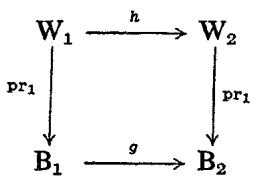
\includegraphics[keepaspectratio]{images/part001_9c3df15b.jpg}}

morphism of class \(\mathbf{C}^{r}\) . Let \(\mathbf{W}_{1}\) (resp. \(\mathbf{W}_{2}\)) be an open subset of \(\mathbf{B}_{1}\times\mathbf{F}_{1}\) (resp. of \(\mathbf{B}_{2}\times\mathbf{F}_{2}\)) and let \(h:\mathbf{W}_{1}\to\mathbf{W}_{2}\) be a map. We say that \(h\) is a \(g\)-morphism of class \(\mathbf{C}^{r,s}\) if \(\mathrm{pr}_{1}\circ h=g\circ\mathrm{pr}_{1}\) and if \(\mathrm{pr}_{2}\circ h\) is a map of class \(\mathbf{C}^{r,s}\) (15.1.6) from \(\mathbf{W}_{1}\) to \(\mathbf{F}_{2}\) .

Similarly, let \(B_{3}\) be a manifold of class \(C^{r}\) , let \(W_{3}\) be an open subset of \(B_{3} \times F_{3}\) , where \(F_{3}\) is a Banach K-space, and let \(g'\) be a morphism of class \(C^{r}\) from \(B_{2}\) to \(B_{3}\) . If h (resp.

\(h^{\prime})\) is a \(g\) -morphism (resp. \(g^{\prime}\) -morphism) of class \(\mathbf{C}^{r,s}\) of \(\mathbf{W}_1\) to \(\mathbf{W}_2\) (resp. of \(\mathbf{W}_2\) to \(\mathbf{W}_3\) ), the composite \(h^{\prime} \circ h\) is a \((g^{\prime} \circ g)\) -morphism of class \(\mathbf{C}^{r,s}\) of \(\mathbf{W}_1\) to \(\mathbf{W}_3\) .

\subsection{\texorpdfstring{Manifold of class \(C^{r,s}\) over a manifold of class \(C^{r}\)}{Manifold of class C\^{}\{r,s\} over a manifold of class C\^{}\{r\}}}

Throughout this section, we denote by B a differentiable manifold of class \(C^{r}\) .

15.2.1. Let X be a set equipped with a map \(p: \mathbf{X} \to \mathbf{B}\) . We call a chart of X over B a triple \(\theta = (\mathbf{V}, \psi, \mathbf{F})\) , where V is a subset of X, F is a Banach space over K, and \(\psi\) is a bijection from V onto an open subset of \(\mathbf{B} \times \mathbf{F}\) such that \(\mathrm{pr}_1 \circ \psi = p|\mathbf{V}\) .

Let \((\theta_{i})_{i\in I} = ((V_{i},\psi_{i},F_{i}))_{i\in I}\) be a family of charts of X over B. We say that the \(\theta_{i}\) are \(C^{r,s}\)-compatible if, for every pair of elements \(i,j\) of I, the following two conditions are satisfied:

\begin{enumerate}
\def\labelenumi{\alph{enumi})}
\item
  \(\psi_i(V_i \cap V_j)\) is open in \(B \times F_i\) and \(\psi_j(V_i \cap V_j)\) is open in \(B \times F_j\) ;
\item
  the map \(\psi_i\circ\psi_j^{-1}\) from \(\psi_j(V_i\cap V_j)\) to \(\psi_i(V_i\cap V_j)\) is an \(\mathrm{Id}_{\mathbf{B}}\)-morphism of class \(\mathbf{C}^{r,s}\) (15.1.7).
\end{enumerate}

A family \(((\mathrm{V}_i,\psi_i,\mathrm{F}_i))_{i\in I}\) of charts of X over B that are \(\mathbf{C}^{r,s}\)-compatible and whose domains \(\mathrm{V}_i\) cover X is called a \(\mathbf{C}^{r,s}\)-atlas of X (over B). Two \(\mathbf{C}^{r,s}\)-atlases are said to be equivalent if their union is again a \(\mathbf{C}^{r,s}\)-atlas; the relation of equivalence between \(\mathbf{C}^{r,s}\)-atlases is an equivalence relation. An equivalence class of \(\mathbf{C}^{r,s}\)-atlases is called a manifold structure of class \(\mathbf{C}^{r,s}\) over B on the set X; when one wishes to specify K, one writes \(\mathbf{C}_{\mathbb{K}}^{r,s}\) instead of \(\mathbf{C}^{r,s}\) . If X is a manifold of class \(\mathbf{C}^{r,s}\) over B, we say that \(p\colon X\to B\) is the projection of X; if \(\theta\) is a chart of X over B, we say that \(\theta\) is a chart of the \(\mathbf{C}^{r,s}\)-manifold X if \(\theta\) belongs to an atlas of the equivalence class defining the structure of X.

Let X be a manifold of class \(C^{r,s}\) over B, with projection p. There exists on X

a differentiable-manifold structure of class \(\mathbf{C}^{r}\), and only one, such that, for every chart \((V,\psi,F)\) of the \(\mathbf{C}^{r,s}\)-manifold X, V is open in X and \(\psi\) is a \(\mathbf{C}^{r}\)-isomorphism of the open submanifold V of X onto the open submanifold \(\psi(V)\) of \(\mathbf{B}\times F\). If one equips X with this structure, the map \(p:X\to B\) is a submersion of class \(\mathbf{C}^{r}\) .

Let \(b \in \mathbf{B}\) and let \(\mathbf{X}_b = p^{-1}(b)\). There exists a K-manifold structure of class \(\mathbf{C}^s\) on \(\mathbf{X}_b\), and only one, such that, for every chart \(\theta = (\mathbf{V}, \psi, \mathbf{F})\) of the \(\mathbf{C}^{r,s}\)-manifold \(\mathbf{X}\), the triple \(\theta_b = (\mathbf{V} \cap \mathbf{X}_b, \operatorname{pr}_2 \circ \psi | (\mathbf{V} \cap \mathbf{X}_b), \mathbf{F})\) is a chart of the manifold \(\mathbf{X}_b\). The differentiable-manifold structure of class \(\mathbf{C}^r\) underlying this structure is induced by the differentiable-manifold structure of class \(\mathbf{C}^r\) on \(\mathbf{X}\) defined above.
